\iffalse
This file is protected by Copyright. Please refer to the COPYRIGHT file
distributed with this source distribution.

This file is part of OpenCPI <http://www.opencpi.org>

OpenCPI is free software: you can redistribute it and/or modify it under the
terms of the GNU Lesser General Public License as published by the Free Software
Foundation, either version 3 of the License, or (at your option) any later
version.

OpenCPI is distributed in the hope that it will be useful, but WITHOUT ANY
WARRANTY; without even the implied warranty of MERCHANTABILITY or FITNESS FOR A
PARTICULAR PURPOSE. See the GNU Lesser General Public License for more details.

You should have received a copy of the GNU Lesser General Public License along
with this program. If not, see <http://www.gnu.org/licenses/>.
\fi

%----------------------------------------------------------------------------------------
% Update the docTitle and docVersion per document
%----------------------------------------------------------------------------------------
\def\docTitle{OpenCPI\\ \bigskip Matchstiq-Z1 Getting Started Guide}
\def\docVersion{1.5}
\def\rccplatform{xilinx13\_3}
\def\radioName{Matchstiq-Z1}
\def\mountPoint{/mnt/}
\def\copyLoc{ATLAS}
%----------------------------------------------------------------------------------------
\def\snippetpath{../../../../../../doc/av/tex/snippets}
% Usage:
% \def\snippetpath{../../../../../doc/av/tex/snippets/}
% % Usage:
% \def\snippetpath{../../../../../doc/av/tex/snippets/}
% % Usage:
% \def\snippetpath{../../../../../doc/av/tex/snippets/}
% \input{\snippetpath/includes}
% From then on, you can use "input" With no paths to get to "snippets"
% You also get all "major" snippets not part of the global LaTeX_Header
% NOTE: If not using the global LaTeX_Header, you need to
% \usepackage{ifthen} to use the \githubio macro

\hyphenation{ANGRY-VIPER} % Tell it where to hyphenate
\hyphenation{Cent-OS} % Tell it where to hyphenate
\hyphenation{install-ation} % Tell it where to hyphenate

\newcommand{\todo}[1]{\textcolor{red}{TODO: #1}\PackageWarning{TODO:}{#1}} % To do notes
\newcommand{\code}[1]{\texttt{#1}} % For inline code snippet or command line
\newcommand{\sref}[1]{Section~\ref{#1}} % To quickly reference a section

% To quickly reference a versioned PDF on github.io
% \def\ocpiversion{1.5.0}
\def\ocpiversion{1.5.0rc4} % TEMPORARY

% This gives a link to github.io document. By default, it puts the filename.
% You can optionally change the link, e.g.
% \githubio{FPGA\_Vendor\_Tools\_Installation\_Guide.pdf} vs.
% \githubio[\textit{FPGA Vendor Tools Installation Guide}]{FPGA\_Vendor\_Tools\_Installation\_Guide.pdf}
% or if you want the raw ugly URL to come out, \githubioURL{FPGA_Vendor_Tools_Installation_Guide.pdf}
\newcommand{\githubio}[2][]{% The default is for FIRST param!
\href{http://opencpi.github.io/releases/\ocpiversion/#2}{\ifthenelse{\equal{#1}{}}{\texttt{#2}}{#1}}}
\newcommand{\githubioURL}[1]{\url{http://opencpi.github.io/releases/\ocpiversion/#1}}

% Fix import paths
\makeatletter
\def\input@path{{\snippetpath/}}
\makeatother

% From then on, you can use "input" With no paths to get to "snippets"
% You also get all "major" snippets not part of the global LaTeX_Header
% NOTE: If not using the global LaTeX_Header, you need to
% \usepackage{ifthen} to use the \githubio macro

\hyphenation{ANGRY-VIPER} % Tell it where to hyphenate
\hyphenation{Cent-OS} % Tell it where to hyphenate
\hyphenation{install-ation} % Tell it where to hyphenate

\newcommand{\todo}[1]{\textcolor{red}{TODO: #1}\PackageWarning{TODO:}{#1}} % To do notes
\newcommand{\code}[1]{\texttt{#1}} % For inline code snippet or command line
\newcommand{\sref}[1]{Section~\ref{#1}} % To quickly reference a section

% To quickly reference a versioned PDF on github.io
% \def\ocpiversion{1.5.0}
\def\ocpiversion{1.5.0rc4} % TEMPORARY

% This gives a link to github.io document. By default, it puts the filename.
% You can optionally change the link, e.g.
% \githubio{FPGA\_Vendor\_Tools\_Installation\_Guide.pdf} vs.
% \githubio[\textit{FPGA Vendor Tools Installation Guide}]{FPGA\_Vendor\_Tools\_Installation\_Guide.pdf}
% or if you want the raw ugly URL to come out, \githubioURL{FPGA_Vendor_Tools_Installation_Guide.pdf}
\newcommand{\githubio}[2][]{% The default is for FIRST param!
\href{http://opencpi.github.io/releases/\ocpiversion/#2}{\ifthenelse{\equal{#1}{}}{\texttt{#2}}{#1}}}
\newcommand{\githubioURL}[1]{\url{http://opencpi.github.io/releases/\ocpiversion/#1}}

% Fix import paths
\makeatletter
\def\input@path{{\snippetpath/}}
\makeatother

% From then on, you can use "input" With no paths to get to "snippets"
% You also get all "major" snippets not part of the global LaTeX_Header
% NOTE: If not using the global LaTeX_Header, you need to
% \usepackage{ifthen} to use the \githubio macro

\hyphenation{ANGRY-VIPER} % Tell it where to hyphenate
\hyphenation{Cent-OS} % Tell it where to hyphenate
\hyphenation{install-ation} % Tell it where to hyphenate

\newcommand{\todo}[1]{\textcolor{red}{TODO: #1}\PackageWarning{TODO:}{#1}} % To do notes
\newcommand{\code}[1]{\texttt{#1}} % For inline code snippet or command line
\newcommand{\sref}[1]{Section~\ref{#1}} % To quickly reference a section

% To quickly reference a versioned PDF on github.io
% \def\ocpiversion{1.5.0}
\def\ocpiversion{1.5.0rc4} % TEMPORARY

% This gives a link to github.io document. By default, it puts the filename.
% You can optionally change the link, e.g.
% \githubio{FPGA\_Vendor\_Tools\_Installation\_Guide.pdf} vs.
% \githubio[\textit{FPGA Vendor Tools Installation Guide}]{FPGA\_Vendor\_Tools\_Installation\_Guide.pdf}
% or if you want the raw ugly URL to come out, \githubioURL{FPGA_Vendor_Tools_Installation_Guide.pdf}
\newcommand{\githubio}[2][]{% The default is for FIRST param!
\href{http://opencpi.github.io/releases/\ocpiversion/#2}{\ifthenelse{\equal{#1}{}}{\texttt{#2}}{#1}}}
\newcommand{\githubioURL}[1]{\url{http://opencpi.github.io/releases/\ocpiversion/#1}}

% Fix import paths
\makeatletter
\def\input@path{{\snippetpath/}}
\makeatother

\documentclass{article}
\iffalse
This file is protected by Copyright. Please refer to the COPYRIGHT file
distributed with this source distribution.

This file is part of OpenCPI <http://www.opencpi.org>

OpenCPI is free software: you can redistribute it and/or modify it under the
terms of the GNU Lesser General Public License as published by the Free Software
Foundation, either version 3 of the License, or (at your option) any later
version.

OpenCPI is distributed in the hope that it will be useful, but WITHOUT ANY
WARRANTY; without even the implied warranty of MERCHANTABILITY or FITNESS FOR A
PARTICULAR PURPOSE. See the GNU Lesser General Public License for more details.

You should have received a copy of the GNU Lesser General Public License along
with this program. If not, see <http://www.gnu.org/licenses/>.
\fi
\author{} % Force author to be blank
%----------------------------------------------------------------------------------------
% Paper size, orientation and margins
%----------------------------------------------------------------------------------------
\usepackage{geometry}
\geometry{
        letterpaper, % paper type
        portrait,    % text direction
        left=.75in,  % left margin
        top=.75in,   % top margin
        right=.75in, % right margin
        bottom=.75in % bottom margin
 }
%----------------------------------------------------------------------------------------
% Header/Footer
%----------------------------------------------------------------------------------------
\usepackage{fancyhdr} \pagestyle{fancy} % required for fancy headers
\renewcommand{\headrulewidth}{0.5pt}
\renewcommand{\footrulewidth}{0.5pt}
\rhead{\small{ANGRYVIPER Team}}
% \rfoot{\thepage}
%----------------------------------------------------------------------------------------
% Appendix packages
%----------------------------------------------------------------------------------------
\usepackage[toc,page]{appendix}
%----------------------------------------------------------------------------------------
% Defined Commands & Renamed Commands
%----------------------------------------------------------------------------------------
\renewcommand{\contentsname}{Table of Contents}
\renewcommand{\listfigurename}{List of Figures}
\renewcommand{\listtablename}{List of Tables}
%----------------------------------------------------------------------------------------
% Various packages
%----------------------------------------------------------------------------------------
\usepackage[usenames,dvipsnames]{xcolor} % for color names see https://en.wikibooks.org/wiki/LaTeX/Colors
\usepackage{hyperref}  % for linking urls and lists
\usepackage{graphicx}  % for including pictures by file
\usepackage{listings}  % for coding language styles
\usepackage{rotating}  % for sideways table
\usepackage{pifont}    % for sideways table
\usepackage{pdflscape} % for landscape view
\usepackage{subfig}
\usepackage{xstring}
\uchyph=0 % Never hyphenate acronyms like RCC (I think this overrides ANGRYVIPER above)
\renewcommand\_{\textunderscore\allowbreak} % Allow words to break/newline on underscores
%----------------------------------------------------------------------------------------
% Table packages
%----------------------------------------------------------------------------------------
\usepackage{longtable} % for long possibly multi-page tables
\usepackage{tabularx} % c=center,l=left,r=right,X=fill
% These define tabularx columns "C" and "R" to match "X" but center/right aligned
\newcolumntype{C}{>{\centering\arraybackslash}X}
\newcolumntype{R}{>{\raggedleft\arraybackslash}X}
\usepackage{float}
\floatstyle{plaintop}
\usepackage[tableposition=top]{caption}
\newcolumntype{P}[1]{>{\centering\arraybackslash}p{#1}}
\newcolumntype{M}[1]{>{\centering\arraybackslash}m{#1}}
%----------------------------------------------------------------------------------------
% Block Diagram / FSM Drawings
%----------------------------------------------------------------------------------------
\usepackage{tikz}
\usetikzlibrary{shapes,arrows,fit,positioning}
\usetikzlibrary{automata} % used for the fsm
%----------------------------------------------------------------------------------------
% Colors Used
%----------------------------------------------------------------------------------------
\usepackage{colortbl}
\definecolor{blue}{rgb}{.7,.8,.9}
\definecolor{ceruleanblue}{rgb}{0.16, 0.32, 0.75}
\definecolor{drkgreen}{rgb}{0,0.6,0}
\definecolor{deepmagenta}{rgb}{0.8, 0.0, 0.8}
\definecolor{cyan}{rgb}{0.0,0.6,0.6}
\definecolor{maroon}{rgb}{0.5,0,0}
%----------------------------------------------------------------------------------------
% VHDL Coding Language Style
% modified from: http://latex-community.org/forum/viewtopic.php?f=44&t=22076
%----------------------------------------------------------------------------------------
\lstdefinelanguage{VHDL}
{
        basicstyle=\ttfamily\footnotesize,
        columns=fullflexible,keepspaces,      % https://tex.stackexchange.com/a/46695/87531
        keywordstyle=\color{ceruleanblue},
        commentstyle=\color{drkgreen},
        morekeywords={
    library,use,all,entity,is,port,in,out,end,architecture,of,
    begin,and, signal, when, if, else, process, end,
        },
        morecomment=[l]--
}
%----------------------------------------------------------------------------------------
% XML Coding Language Style
% modified from: http://tex.stackexchange.com/questions/10255/xml-syntax-highlighting
%----------------------------------------------------------------------------------------
\lstdefinelanguage{XML}
{
        basicstyle=\ttfamily\footnotesize,
        columns=fullflexible,keepspaces,
        morestring=[s]{"}{"},
        morecomment=[s]{!--}{--},
        commentstyle=\color{drkgreen},
        moredelim=[s][\color{black}]{>}{<},
        moredelim=[s][\color{cyan}]{\ }{=},
        stringstyle=\color{maroon},
        identifierstyle=\color{ceruleanblue}
}
%----------------------------------------------------------------------------------------
% DIFF Coding Language Style
% modified from http://tex.stackexchange.com/questions/50176/highlighting-a-diff-file
%----------------------------------------------------------------------------------------
\lstdefinelanguage{diff}
{
        basicstyle=\ttfamily\footnotesize,
        columns=fullflexible,keepspaces,
        breaklines=true,                                % wrap text
        morecomment=[f][\color{ceruleanblue}]{@@},      % group identifier
        morecomment=[f][\color{red}]-,                  % deleted lines
        morecomment=[f][\color{drkgreen}]+,             % added lines
        morecomment=[f][\color{deepmagenta}]{---},      % Diff header lines (must appear after +,-)
        morecomment=[f][\color{deepmagenta}]{+++},
}
%----------------------------------------------------------------------------------------
% Python Coding Language Style
% modified from
%----------------------------------------------------------------------------------------
\lstdefinelanguage{python}
{
        basicstyle=\ttfamily\footnotesize,
        columns=fullflexible,keepspaces,
        keywordstyle=\color{ceruleanblue},
        commentstyle=\color{drkgreen},
        stringstyle=\color{orange},
        morekeywords={
    print, if, sys, len, from, import, as, open,close, def, main, for, else, write, read, range,
        },
        comment=[l]{\#}
}
%----------------------------------------------------------------------------------------
% Fontsize Notes in order from smallest to largest
%----------------------------------------------------------------------------------------
%    \tiny
%    \scriptsize
%    \footnotesize
%    \small
%    \normalsize
%    \large
%    \Large
%    \LARGE
%    \huge
%    \Huge

\iffalse
This file is protected by Copyright. Please refer to the COPYRIGHT file
distributed with this source distribution.

This file is part of OpenCPI <http://www.opencpi.org>

OpenCPI is free software: you can redistribute it and/or modify it under the
terms of the GNU Lesser General Public License as published by the Free Software
Foundation, either version 3 of the License, or (at your option) any later
version.

OpenCPI is distributed in the hope that it will be useful, but WITHOUT ANY
WARRANTY; without even the implied warranty of MERCHANTABILITY or FITNESS FOR A
PARTICULAR PURPOSE. See the GNU Lesser General Public License for more details.

You should have received a copy of the GNU Lesser General Public License along
with this program. If not, see <http://www.gnu.org/licenses/>.
\fi

\iffalse

This snippet defines macros to be used when describing ocpidev commands
to give the user the equivalent in the IDE. See AV-4628.

To see all output:
\code{\$ ocpidev build something something}
\OcpidevBuild
\code{\$ ocpidev clean something something}
\OcpidevClean
\code{\$ ocpidev run test something something}
\OcpidevRunTest
\code{\$ ocpidev create (no options)}
\OcpidevCreate{}
\code{\$ ocpidev create project}
\OcpidevCreate{Project}
\code{\$ ocpidev clean project Project}
\OcpidevCleanProject{Project}
\code{\$ ocpidev register project my\_proj}
\OcpidevRegisterProject{my_proj}
\code{\$ ocpidev unregister project my\_proj}
\OcpidevUnRegisterProject{my_proj}

\fi
% https://tex.stackexchange.com/a/5227
\usetikzlibrary{shadows}
\newcommand*\OcpidevKeystroke[1]{%
  \tikz[baseline=(key.base)]
    \node[%
      draw,
      fill=white,
      drop shadow={shadow xshift=0.25ex,shadow yshift=-0.25ex,fill=black,opacity=0.75},
      rectangle,
      rounded corners=2pt,
      inner sep=1pt,
      line width=0.5pt,
      font=\scriptsize\sffamily
    ](key) {#1\strut}
  ;
}

\providecommand{\OcpidevCtrlClick}{(use \OcpidevKeystroke{~Ctrl~} for multiple selection)}

\providecommand{\OcpidevTemplate}[1]{
\begin{center}
\framebox{\parbox{0.8\linewidth}{\textit{To perform this operation within the IDE:}
#1}}
\end{center}
}

% OcpidevBuild = "ocpidev build"
\providecommand{\OcpidevBuild}{\OcpidevTemplate{
\begin{enumerate}
\setlength\itemsep{0em} %tighten
\item Open the ANGRYVIPER Perspective
\item Select the asset from OpenCPI Project View
\item Import to ANGRYVIPER Operations Panel using ``$>$'' button
\item Select the RCC and/or HDL platforms for the build \OcpidevCtrlClick
\item Click ``Build''
\end{enumerate}
% Open the ANGRYVIPER Perspective, select the RCC and/or HDL platforms for the build \OcpidevCtrlClick , then select the asset in OpenCPI Projects view, right click, select build.
}}

% OcpidevClean = "ocpidev clean"
\providecommand{\OcpidevClean}{\OcpidevTemplate{
In the OpenCPI Projects view, select the project, right-click, select clean from the menu.
}}

% OcpidevRunTest = "ocpidev run test"
\providecommand{\OcpidevRunTest}{\OcpidevTemplate{
\begin{enumerate}
\setlength\itemsep{0em} %tighten
\item Click the ``Tests'' radio button and select RCC and/or HDL platforms for the run \OcpidevCtrlClick .
\item Click the ``+remotes'' button, enter the remote string, click OK.
\item Select the remote in the remotes list.
\item In the OpenCPI Projects view, select the desired unit tests, click the ``$>$'' button in the operations panel, then click the desired operation to build and then run the listed tests on the selected remote.
\end{enumerate}
}}

% OcpidevCreate = "ocpidev create <$1>"
\providecommand{\OcpidevCreate}[1]{\OcpidevTemplate{
\begin{itemize}
\setlength\itemsep{0em} %tighten
\item Place the cursor in the OpenCPI Projects panel, right click, select asset wizard.
\item Select the asset type\ifthenelse{\equal{#1}{}}{}{ (``#1'')} in the drop-down, fill in the required inputs, click finish.
\item When the process finishes, the new asset is displayed in both project views. (If the asset has an XML editor, then the editor opens.)
\end{itemize}
}}

% OcpidevCleanProject = "ocpidev clean project <$1>"
\providecommand{\OcpidevCleanProject}[1]{\OcpidevTemplate{\textit{(The project ``#1'' must be imported into the IDE and then refresh the OpenCPI Projects view so the project is shown.)}
\begin{itemize}
\setlength\itemsep{0em} %tighten
\item Right click on #1 $\Rightarrow$ ``Clean''
\end{itemize}
}}

% OcpidevRegisterProject = "ocpidev register project <$1>"
% OcpidevUnRegisterProject = "ocpidev unregister project <$1>"
\providecommand{\OcpidevRegisterProjectKernel}[2]{\OcpidevTemplate{\textit{(The project ``#1'' must be imported into the IDE and then refresh the OpenCPI Projects view so the project is shown.)}
\begin{itemize}
\setlength\itemsep{0em} %tighten
\item In the OpenCPI Projects view, select the project, right-click, select ``#2'' from the menu. (Depending on state of the project, this option may not be available.)
\end{itemize}
}}
\providecommand{\OcpidevRegisterProject}[2]{\OcpidevRegisterProjectKernel{\path{#1}}{register}}
\providecommand{\OcpidevUnRegisterProject}[2]{\OcpidevRegisterProjectKernel{\path{#1}}{unregister}}

\date{Version \docVersion} % Force date to be blank and override date with version
\title{\docTitle}
\lhead{Matchstiq-Z1 Getting Started Guide}
%----------------------------------------------------------------------------------------
\usepackage[T1]{fontenc} % http://tex.stackexchange.com/a/181119
\usepackage{graphicx}
\graphicspath{ {figures/} }
\lstset{ % https://tex.stackexchange.com/a/116572
  basicstyle=\ttfamily,
  columns=fullflexible,
  % frame=single,
  breaklines=true,
  showstringspaces=true,
  showspaces=true,
  postbreak=\mbox{\textcolor{red}{$\hookrightarrow$}\space},
}
\usepackage{textcomp}
\begin{document}
\maketitle
%\thispagestyle{fancy}

\newpage

	\begin{center}
	\textit{\textbf{Revision History}}
		\begin{table}[H]
		\label{table:revisions} % Add "[H]" to force placement of table
			\begin{tabularx}{\textwidth}{|c|X|l|}
			\hline
			\rowcolor{blue}
			\textbf{Revision} & \textbf{Description of Change} & \textbf{Date} \\
		    \hline
            v1.1 & Initial Release & 3/2017 \\
            \hline
            v1.2 & Updated for OpenCPI Release 1.2 & 8/2017 \\
            \hline
            v1.3 & Updated for OpenCPI Release 1.3 & 2/2018 \\
            \hline
            v1.4 & Update descriptions and paths & 9/2018 \\
            \hline
            v1.5 & Update  for OpenCPI Release 1.5 & 4/2019 \\
            \hline
			\end{tabularx}
		\end{table}
	\end{center}

\newpage

\tableofcontents

\newpage

\section{References}

	This document assumes a basic understanding of the Linux command line (or ``shell'') environment.  The reference(s) in Table 1 can be used as an overview of OpenCPI and may prove useful.
\def\refskipocpiov{}
\def\refcapbottom{}
\iffalse
This file is protected by Copyright. Please refer to the COPYRIGHT file
distributed with this source distribution.

This file is part of OpenCPI <http://www.opencpi.org>

OpenCPI is free software: you can redistribute it and/or modify it under the
terms of the GNU Lesser General Public License as published by the Free Software
Foundation, either version 3 of the License, or (at your option) any later
version.

OpenCPI is distributed in the hope that it will be useful, but WITHOUT ANY
WARRANTY; without even the implied warranty of MERCHANTABILITY or FITNESS FOR A
PARTICULAR PURPOSE. See the GNU Lesser General Public License for more details.

You should have received a copy of the GNU Lesser General Public License along
with this program. If not, see <http://www.gnu.org/licenses/>.
\fi

% This snippet creates the "References" table labeled "table:references"
% It creates three columns: Name, Publisher, Link and then inserts default documents
%
% To skip these defaults, define macros named
% refskipgs to skip "Getting Started"
% refskipig to skip "Installation Guide"
% refskipac to skip "Acronyms and Definitions"
% refskipocpiov to skip "OpenCPI Overview"
%
% See RPM_Installation_Guide.tex for examples
%
% After the defaults, it optionally inserts the "myreferences" macro that
% you defined elsewhere (you put hlines above all lines)
%
% If you want the \caption on the bottom, define "refcapbottom"
\begin{center}
\renewcommand*\footnoterule{} % Remove separator line from footnote
\renewcommand{\thempfootnote}{\arabic{mpfootnote}} % Use Arabic numbers (or can't reuse)
\begin{minipage}{0.9\textwidth}
  \begin{table}[H]
\ifx\refcapbottom\undefined
  \caption {References}
  \label{table:references}
\fi
  \begin{tabularx}{\textwidth}{|C|C|}
    \hline
    \rowcolor{blue}
    \textbf{Title} & \textbf{Link} \\
\ifx\refskipocpiov\undefined
    \hline
    OpenCPI Overview & \githubio{Overview.pdf} \\
\fi
\ifx\refskipac\undefined
    \hline
    Acronyms and Definitions & \githubio{Acronyms\_and\_Definitions.pdf} \\
\fi
\ifx\refskipgs\undefined
    \hline
    Getting Started & \githubio{Getting\_Started.pdf} \\
\fi
\ifx\refskipig\undefined
    \hline
    Installation Guide & \githubio{RPM\_Installation\_Guide.pdf} \\
\fi
\ifx\myreferences\undefined
\else
    \myreferences
\fi
    \hline
  \end{tabularx}
\ifx\refcapbottom\undefined
\else
  \caption {References}
  \label{table:references}
\fi
  \end{table}
\end{minipage}
\end{center}


\newpage
\section{Overview}
This document provides steps for configuring a factory provided Epiq Solutions Matchstiq-Z1 SDR with the OpenCPI run-time environment for executing applications, configuring a development system to build OpenCPI bitstreams targeting the \textit{matchstiq\_z1} platform, and examples of executing applications on the OpenCPI configured Matchstiq-Z1. \textbf{Note: Only the Z1 version of the Epiq Solutions Matchstiq product line is supported by OpenCPI.}

\section{Prerequisites}
\begin{flushleft}
This guide assumes that, at a minimum, the following RPMs are installed:  \\
\begin{table}[H]
	\label{table:rpms}
		\begin{tabularx}{\textwidth}{|c|X|}
		\hline
		\rowcolor{blue}
		\textbf{RPM Name} & \textbf{Description} \\
		\hline
		\hline
		All prerequisite RPMs & These packages have OpenCPI-specific patches and are provided as RPMs. This packaging ensures they will not conflict with other installed copies by using a nonstandard installation location of \path{/opt/opencpi/prerequisites}. \\
		\hline
		\small{\code{angryviper-ide-*.x86 64.rpm}} &
		The ANGRYVIPER IDE (Eclipse with plugins). See RPM Installation Guide.pdf, Appendix D for an alternative method to set up the IDE using an existing Eclipse installation. \\
		\hline
		\small{\code{opencpi-*.x86\_64.rpm}} &
		Base installation RPM includes the runtime portion of the Component
Development Kit (CDK) and the source for the ocpi.core and ocpi.assets Projects containing framework essential components, workers,
platforms, etc. \\
		\hline
		\small{\code{opencpi-devel-*.x86\_64.rpm}} &
		Additional header files and scripts for developing new assets as HDL
and/or RCC. \\
		\hline
		\small{\code{opencpi-sw-platform-xilinx13\_3-*.noarch.rpm}} &
		Additional files necessary to build the framework targeting specific
RCC/software platforms, independent of the final deployed hardware. \\
		\hline
		\small{\code{opencpi-hw-platform-matchstiq\_z1-xilinx13\_3-*.noarch.rpm}} &
		Additional files necessary to build the framework targeting specific hard-ware platform ``X'' when running RCC platform ``Y'' (``Y'' can be ``no sw''). This RPM also includes hardware-specific SD Card images when applicable. \\
		\hline
	\end{tabularx}
\end{table}

\subsection{Installation of provided OpenCPI projects: \textit{core} and \textit{assets}}
This guide  assumes the user has executed \textit{ocpi-copy-projects}, accepting the default settings, to copy and register the \textit{core} and \textit{assets} projects from the /opt/opencpi/projects for building bitstreams for the Matchstiq-Z1. Reference the Getting Started Guide for details on \textit{ocpi-copy-projects}.  While registering of the projects is performed during the execution of ocpi-copy-projects, changes to the registry can be made via \code{ocpidev un/register project} or the ANGRYVIPER GUI.\medskip

\begin{verbatim}
$ ocpi-copy-projects
...

$ ls ~/ocpi_projects
assets core
$ ocpidev show registry
Project registry is located at: /opt/opencpi/cdk/../project-registry
----------------------------------------------------------------------------------------
| Project Package-ID  | Path to Project                                 | Valid/Exists |
| ------------------  | ---------------                                 | ------------ |
| ocpi.core           | /home/user/ocpi_projects/core                   | True         |
| ocpi.assets         | /home/user/ocpi_projects/assets                 | True         |
----------------------------------------------------------------------------------------
\end{verbatim}

\subsection{Vendor Software Setup}
The platform that is expected to be used is the Epiq Solutions Matchstiq-Z1 (\textit{e.g.} matchstiq\_z1). This OpenCPI-enabled platform provides the capability of deploying hardware and software workers while using Xilinx's 13.3 distribution of Linux.\\ \bigskip

The synthesizers and cross-compilers required to build HDL and RCC Workers for this platform are installed by following the instructions found in the \textit{OpenCPI FPGA Vendor Tools Installation Guide}. This document assumes that the user has installed the appropriate versions of Vivado and the Xilinx SDK.\\ \bigskip

\subsection{Building OpenCPI projects: \textit{core} and \textit{assets} }
\label{sec:Building OpenCPI projects}
The \textit{core} and \textit{assets} projects must be built \textit{in a specific order} for this platform. This section outlines how to build the relevant projects and provides the commands to do so.\medskip

For this document, the projects should be built as follows:\\

\begin{enumerate}
	\item Build \code{core} for the \code{xilinx13\_3} RCC Platform and the \code{matchstiq\_z1} HDL Platform (approx 30 min)
	\item Build \code{assets} for the \code{xilinx13\_3} RCC Platform and the \code{matchstiq\_z1} HDL Platform, but omit assemblies (approx 45 min)
	\item Build the \code{testbias} assembly from the \code{assets} project. This will be used later in this guide. (approx 10 min)
\end{enumerate}
\begin{lstlisting}[showspaces=false]
$ cd /home/<user>/ocpi_projects/
$ ocpidev build -d core     --rcc-platform xilinx13_3 --hdl-platform matchstiq_z1
$ ocpidev build -d assets   --rcc-platform xilinx13_3 --hdl-platform matchstiq_z1 --no-assemblies
$ ocpidev build -d assets hdl assembly testbias       --hdl-platform matchstiq_z1
\end{lstlisting}
Note: replace ``\code{<user>}'' with your username in the commands above.\\\medskip

Each of these build commands can also be performed via the ANGRYVIPER IDE as follows:
\OcpidevBuild
See the ANGRYVIPER Team's Getting Started Guide for additional information concerning the use of \code{ocpidev} and the ANGRYVIPER IDE to build OpenCPI assets.

\subsection{Hardware Setup}
\begin{itemize}

\item \textbf{Epiq Solutions Matchstiq-Z1 SDR Kit}\\ \medskip
It is expected that this SDR kit includes a power supply, two SMA/SMB adapters, micro-USB to USB cable, micro-SD card installed internally (expected).

A micro-USB connector on the back of the Matchstiq-Z1 provides access to the serial connection. To expose this micro-USB connector, the two screws in the back plate must be removed.  Historically, this connector's attachment to the PCB has been extremely fragile, \textbf{so be careful when inserting/removing the mating cable}.\\ \medskip

\begin{figure}[ht]
	\centerline{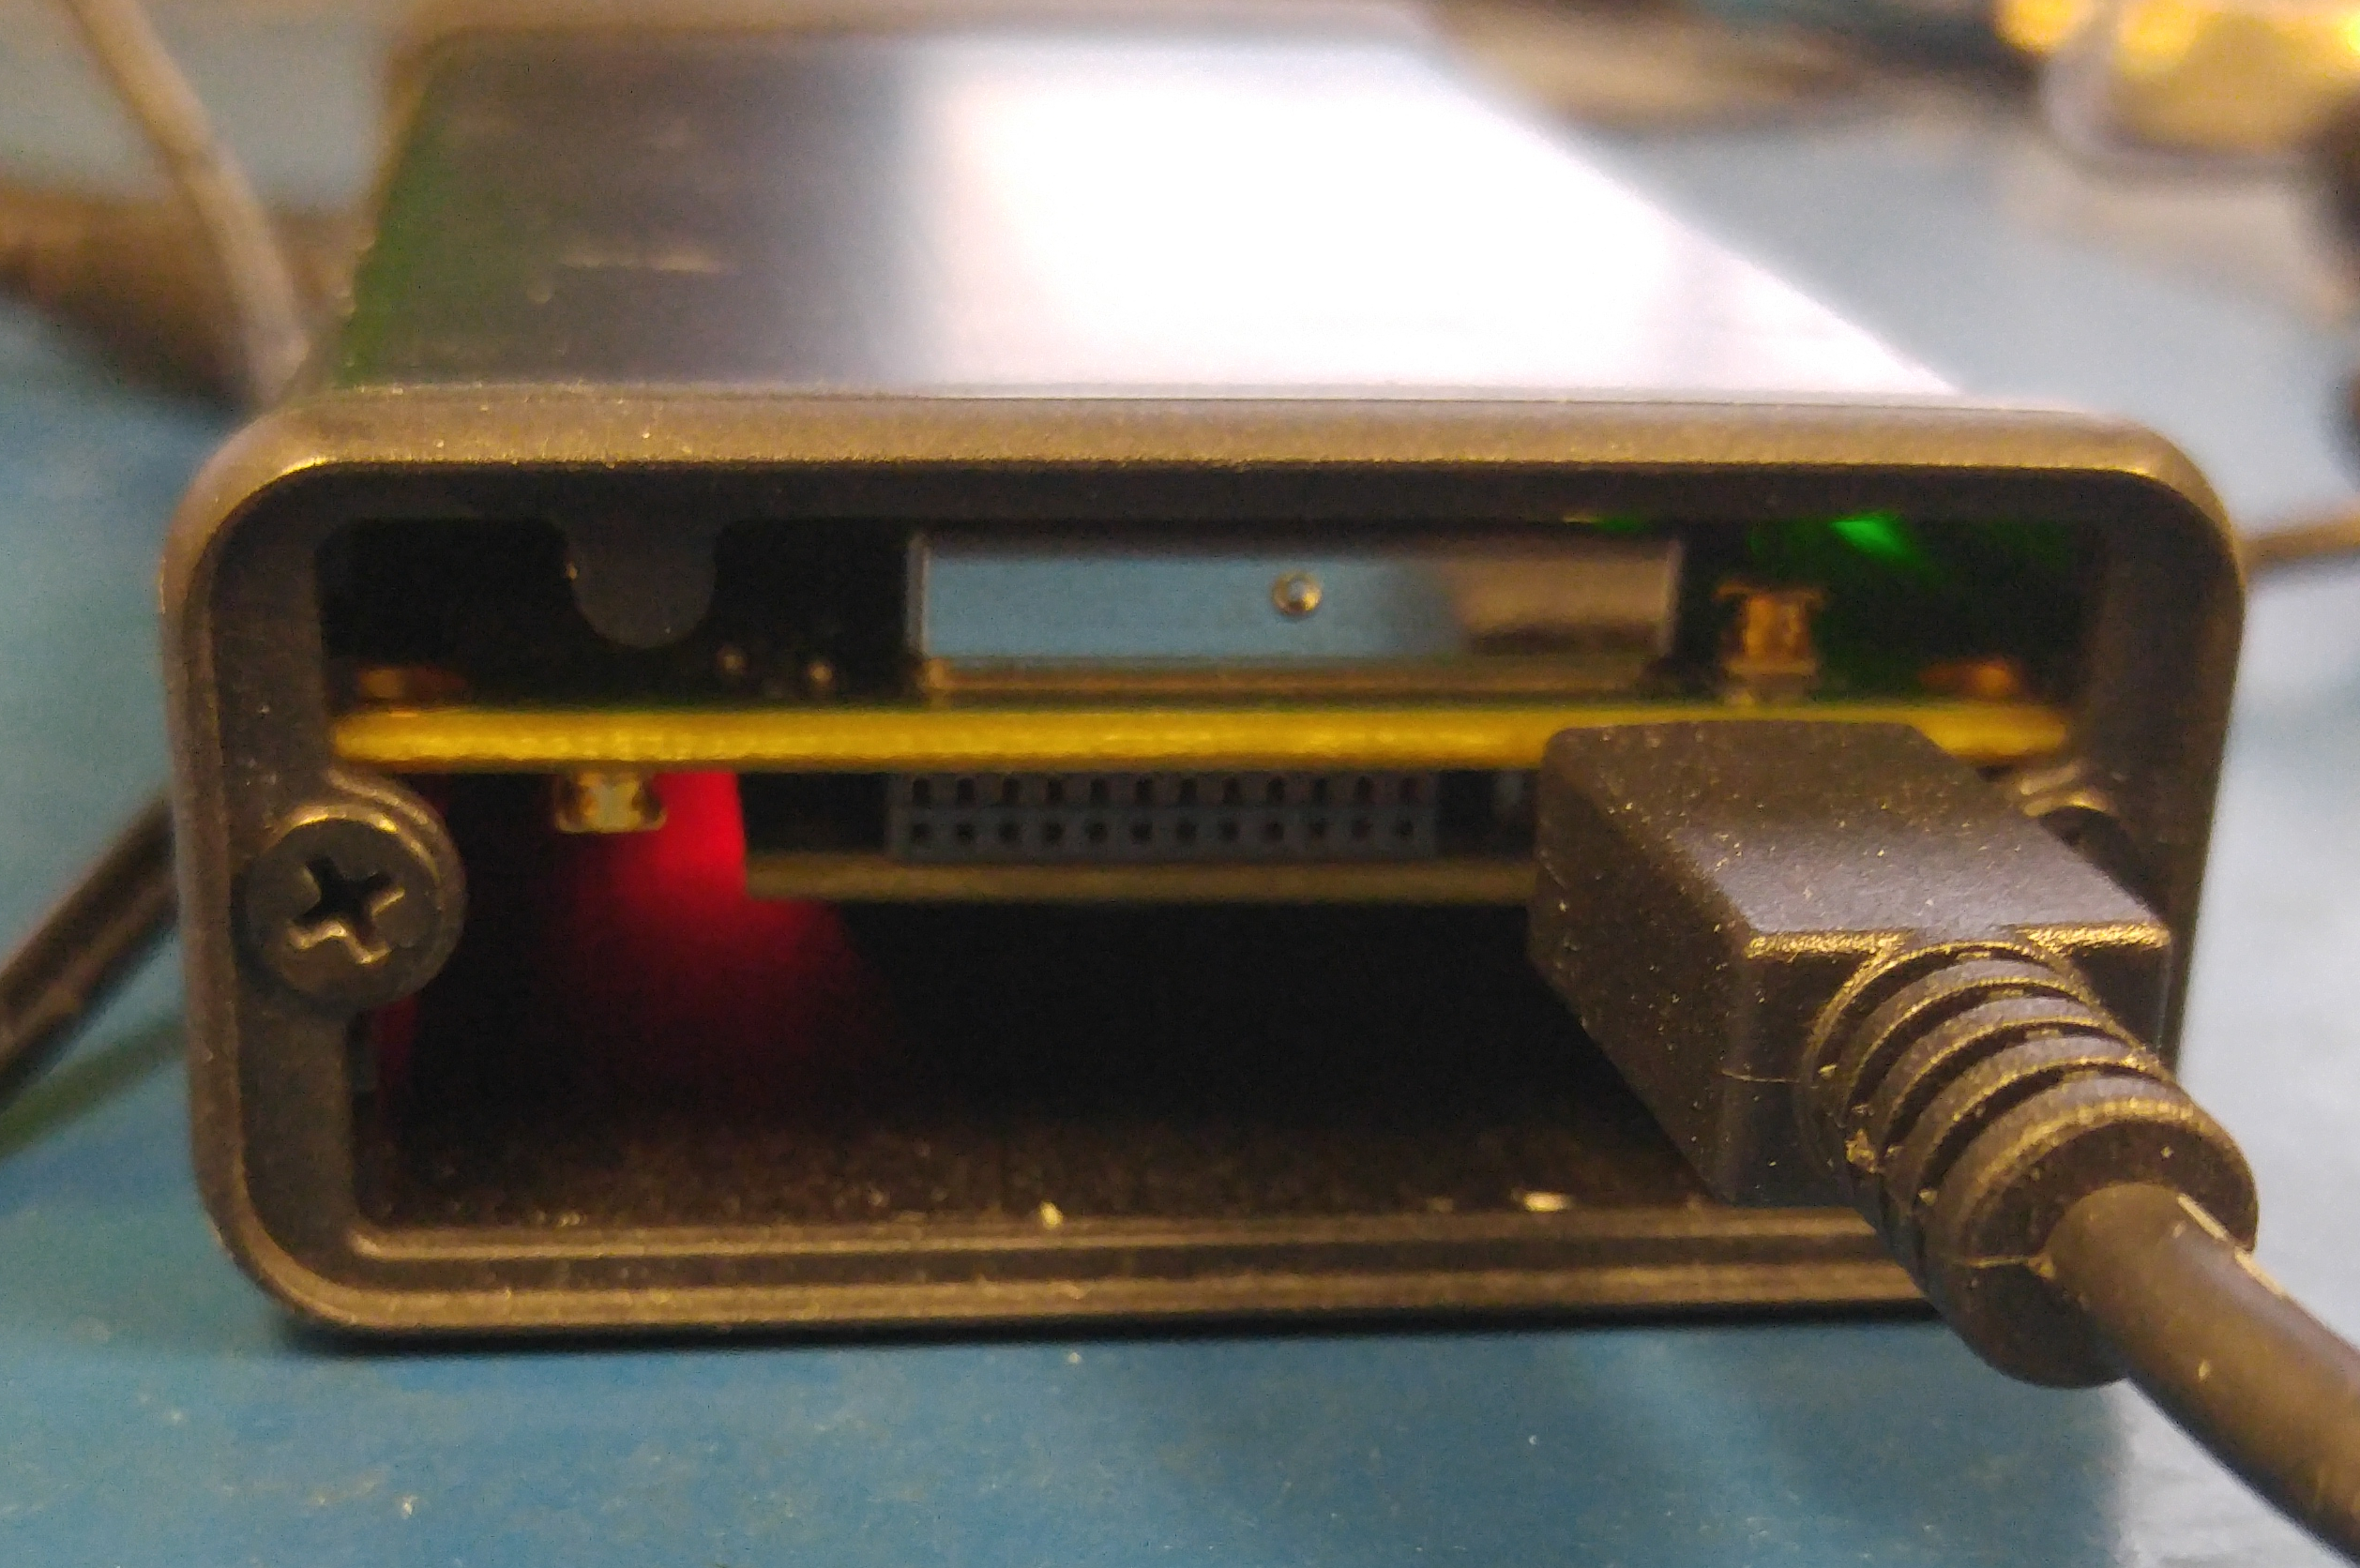
\includegraphics[scale=0.08]{Matchstiq_Z1_backpannel}}
	\caption{Connected Back Panel}
	\label{fig:back}
\end{figure}

\item \textbf{Micro-USB to Ethernet adapter}. To allow network access when plugged into the front panel micro-USB port.  The OpenCPI BSP for the Matchstiq-Z1 is configured for DHCP. An Ethernet connection is required for developing OpenCPI in Network mode.

On the front panel of the Matchstiq-Z1, there are three labeled SMB (50 Ohm) connectors: ``RX'' (receive), ``TX'' (transmit), and ``GPS''.  From the factory, the Matchstiq-Z1 is provided with two SMB to SMA adapters.  Due to the RF performance to the transceiver device, any RF COAX cables should be rated up to at least 3GHz. \\ \medskip
\begin{figure}[ht]
	\centerline{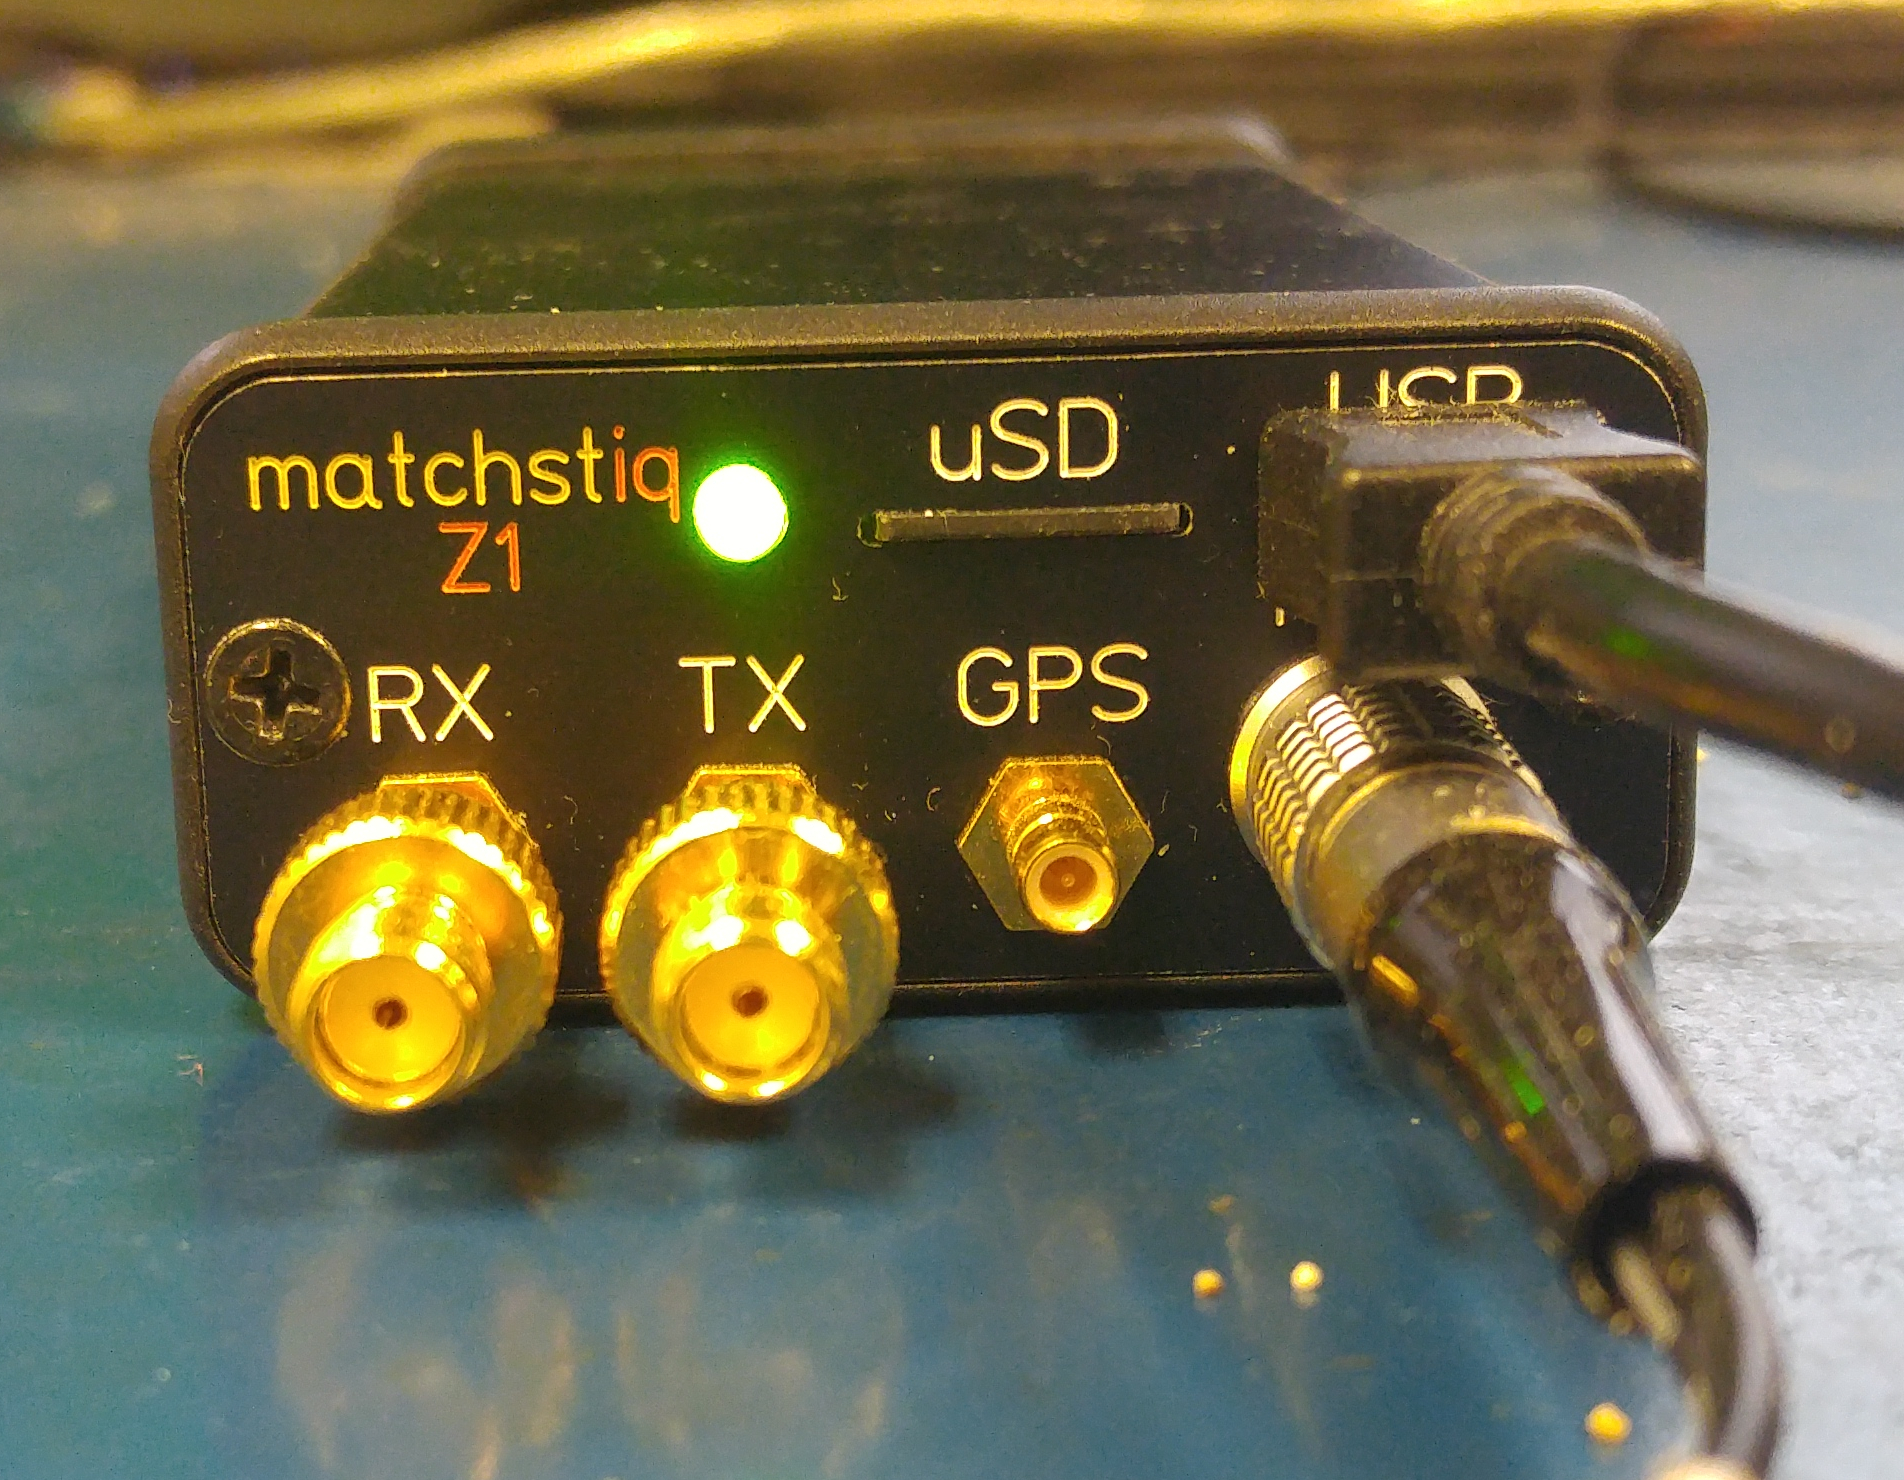
\includegraphics[scale=0.1]{Matchstiq_Z1_frontpannel}}
	\caption{Connected Front Panel}
	\label{fig:front}
\end{figure}

\item \textbf{Access to a network which supports DHCP. (Network Mode)}
\item \textbf{Micro-SD card, 4GB+ (OPTIONAL, as it is possible to use internally installed card) }
\item \textbf{Micro-SD card reader}
\end{itemize}
\end{flushleft}

\newpage
\section{SD Card Setup}
\label{sec:SD_Card_Setup}
The Matchstiq-Z1 SDR is equipped with two SD card slots: one internal and one accessible via the front panel. It is expected that the SDRs are shipped from Epiq Solutions with an SD card installed in the internal slot that is loaded with their embedded environment. A feature of this SDR is that when an SD card is installed in the front panel SD slot, the SDR will automatically choose to operate from this SD card rather than the internal SD card. Therefore, a user can easily switch the SDR between operating in the Epiq Solutions or OpenCPI environment.

The Matchstiq-Z1's factory SD card has a non-default formatting and content, which \textit{must} be maintained for proper operation. This guide assumes that the internal (factory) SD card is being use for OpenCPI and will be reinstalled in the front panel SD card slot. If the user desires the use of a new SD card, the user must ensure that it is initially imaged from the factory provided SD card, as there is a unique partition containing required content from the OEM.

\subsection{Make a backup image of factory SD card (assumes Linux host)}
This section provides the steps for creating an SD card backup image.  Access the internal SD card slot by removing the screws from the front and back plates, then slide the board assembly out of the enclosure. Flip the SD card slot open and lift the card out. Insert the SD card into a USB reader and install into a host machine.
\begin{enumerate}
	\item Determine the device file name for the SD card by
	executing dmesg command below. It will likely be something
	like \texttt{/dev/sdb} or \texttt{/dev/mmcblk0}.\\ \\
	\texttt{\$ dmesg | tail -n 15}
	\item Run the following \textit{dd} command to make a backup
	image, where DEVICENAME was determined above. This step
	should take $\sim15$ minutes depending on the card size.\\ \\
	\texttt{\$ dd if=DEVICENAME of=backup.image}
\end{enumerate}

\subsection{Format the SD card for OpenCPI}
The Matchstiq-Z1 SDR requires an SD card with a
specific partition and content. The recommend method for formatting a new SD card is to begin by imaging the new card using the backup image of the factory SD card, removing factory default files and directory and copying OpenCPI content to SD card.
\begin{enumerate}
	\item Format an SD card for OpenCPI, (restore to its original factory default captured in the previous section), run the command \\ \\
	\texttt{\$ dd of=DEVICENAME if=backup.image}
	\item To prepare for OpenCPI provided content to be placed onto the SD card, remove all factory files and directories from the ATLAS partition.
\end{enumerate}

\subsection{Copy embedded OS files to SD card, ``ATLAS'' partition}
\label{sec:Copy embedded OS to SD card}
\begin{flushleft}

WARNING: The user must ensure that the contents of the SD, match the version of the OpenCPI release that the artifacts were built against.\\ \medskip

Copy the following files/directories into the ``ATLAS'' partition:
\begin{verbatim}
$ cp /opt/opencpi/cdk/matchstiq_z1/sdcard-xilinx13_3/iveia-atlas-i-z7e.dtb /run/media/<user>/ATLAS/

$ cp /opt/opencpi/cdk/matchstiq_z1/sdcard-xilinx13_3/u-boot.bin /run/media/<user>/ATLAS/

$ cp /opt/opencpi/cdk/matchstiq_z1/sdcard-xilinx13_3/uImage /run/media/<user>/ATLAS/

$ cp /opt/opencpi/cdk/matchstiq_z1/sdcard-xilinx13_3/uramdisk.image.gz /run/media/<user>/ATLAS/
\end{verbatim}

Any files/directories copied to the ``ATLAS'' partition will appear at /mnt/card on the Matchstiq-Z1.\\ \medskip

The need to copy the \textit{/opt/opencpi/cdk/matchstiq\_z1/opencpi} onto the SD card is dependent on the desired operating mode (Standalone vs Network) and is discussed in the following sections.
\end{flushleft}

\subsection{Copy files to SD card for desired Mode(s)}
As previously discussed, Standalone and Network modes offer trade-offs for configuring the run-time environment of the platform. The following sections provide instructions for copying specific files/directories to the SD card in support of these modes. For maximum flexibility and completion of this getting started guide, it is recommended that the SD card be configured to support both modes, as covered in the next sub-section. However, instructions for configuring the SD card for each mode separately, have also been provided.

\subsubsection{Standalone and Network Modes}
The SD can be setup to support both modes, as there is no conflict between the files/directories for either mode. To setup the SD to support both modes:\\

\noindent After performing the steps from \ref{sec:Copy embedded OS to SD card}, copy the entire \textit{opencpi} directory to the SD card.

\begin{verbatim}
$ cp -rL /opt/opencpi/cdk/matchstiq_z1/sdcard-xilinx13_3/opencpi /run/media/<user>/ATLAS/

$ cp /home/<user>/ocpi_projects/assets/hdl/assemblies/testbias/container-testbias_matchstiq_z1_base/\
target-zynq/testbias_matchstiq_z1_base.bit.gz /run/media/<user>/ATLAS/opencpi/xilinx13_3/artifacts/
\end{verbatim}

\subsubsection{Standalone Mode}
After performing the steps from \ref{sec:Copy embedded OS to SD card}, copy the entire \textit{opencpi} directory to the SD card, then copy the relevant bitstreams, artifacts into the \textit{artifacts} directory and application XMLs into the \textit{applications} directory. For this getting started guide, only one bitstream is required to be copied onto the SD cards, where as the required artifacts and application XML where copied to the SD along with the entire \textit{opencpi} directory.

\begin{verbatim}
$ cp -rL /opt/opencpi/cdk/matchstiq_z1/sdcard-xilinx13_3/opencpi /run/media/<user>/ATLAS/

$ cp /home/<user>/ocpi_projects/assets/hdl/assemblies/testbias/container-testbias_matchstiq_z1_base/\
target-zynq/testbias_matchstiq_z1_base.bit.gz /run/media/<user>/ATLAS/opencpi/xilinx13_3/artifacts/
\end{verbatim}

\subsubsection{Network Mode}
After performing the steps from \ref{sec:Copy embedded OS to SD card}, create a directory on the partition named ``opencpi'' and copy the following files into the this directory:

\begin{verbatim}
$ mkdir /run/media/<user>/ATLAS/opencpi

$ cp /opt/opencpi/cdk/matchstiq_z1/sdcard-xilinx13_3/opencpi/system.xml \
/run/media/<user>/ATLAS/opencpi/

$ cp /opt/opencpi/cdk/matchstiq_z1/sdcard-xilinx13_3/opencpi/default_mynetsetup.sh \
/run/media/<user>/ATLAS/opencpi/

$ cp /opt/opencpi/cdk/matchstiq_z1/sdcard-xilinx13_3/opencpi/zynq_net_setup.sh \
/run/media/<user>/ATLAS/opencpi/
\end{verbatim}

\subsection{SD Card Source}
The final SD Card artifacts are distributed in \path{/opt/opencpi/cdk/matchstiq_z1/} via RPM as noted previously. The end user is not required nor expected to generate the files.

\subsection{No changes required for ``SDHOME'' partition}
All the files in this partition can be ignored. If space for files is required for your application, they can be deleted.


\pagebreak

\iffalse
This file is protected by Copyright. Please refer to the COPYRIGHT file
distributed with this source distribution.

This file is part of OpenCPI <http://www.opencpi.org>

OpenCPI is free software: you can redistribute it and/or modify it under the
terms of the GNU Lesser General Public License as published by the Free Software
Foundation, either version 3 of the License, or (at your option) any later
version.

OpenCPI is distributed in the hope that it will be useful, but WITHOUT ANY
WARRANTY; without even the implied warranty of MERCHANTABILITY or FITNESS FOR A
PARTICULAR PURPOSE. See the GNU Lesser General Public License for more details.

You should have received a copy of the GNU Lesser General Public License along
with this program. If not, see <http://www.gnu.org/licenses/>.
\fi


\section{Script Setup}
There are two type of setups or modes for running applications on any embedded radio: Network and Standalone. In Network mode, a development system hosts the OpenCPI tree as an NFS server to the \radioName \space which is an NFS client. This configuration provides quick and dynamic access to all of OpenCPI, and presumably any applications, components and bitstreams. In Standalone mode, all the artifacts are located on the SDR's local storage (\textit{e.g.} SD card) and no network connection is required. This may be more suited for \textit{deployment} scenarios in which network connection is not possible or practical. Network mode is generally preferred during the development process.

\begin{flushleft}

\subsection{Setting up the Network and Standalone Mode scripts}

For each mode, a startup script is used to configure the environment of the embedded system. The OpenCPI framework provides a default script for each mode. The default scripts are to be copied and modified per the user's requirements.\par\medskip

\subsubsection{Network Mode}
1) Make a copy of the default script for editing. \\ \medskip
\begin{texttt}
\$ cp /run/media/<user>/\copyLoc/opencpi/default\_mynetsetup.sh \textbackslash\\
/run/media/<user>/\copyLoc/opencpi/mynetsetup.sh
\end{texttt}\medskip

2) Edit the copy
\begin{enumerate}
\item In \texttt{mynetsetup.sh}, uncomment the following lines which are necessary for mounting \textit{core} and \textit{assets} project: \\ \medskip

\begin{texttt}
mkdir -p \mountPoint ocpi\_core \\
mount -t nfs -o udp,nolock,soft,intr \$1:/home/user/ocpi\_projects/core \mountPoint ocpi\_core \\
mkdir -p \mountPoint ocpi\_assets \\
mount -t nfs -o udp,nolock,soft,intr \$1:/home/user/ocpi\_projects/assets \mountPoint ocpi\_assets\\
\end{texttt}
 \item Edit \texttt{/home/user/ocpi\_projects/core} and \texttt{/home/user/ocpi\_projects/assets} to reflect the paths to the \textit{core} and \textit{assets} project on the host, e.g.:\\ \medskip
\begin{texttt}
mkdir -p \mountPoint ocpi\_core \\
mount -t nfs -o udp,nolock,soft,intr \$1:/home/johndoe/ocpi\_projects/core \mountPoint ocpi\_core\\
mkdir -p \mountPoint ocpi\_assets \\
mount -t nfs -o udp,nolock,soft,intr \$1:/home/johndoe/ocpi\_projects/assets \mountPoint ocpi\_assets\\
\end{texttt}
\ifx\bspProj\undefined
%do nothing 
\else 
\begin{texttt}
mkdir -p \mountPoint \bspProj \\
mount -t nfs -o udp,nolock,soft,intr \$1:/home/johndoe/ocpi\_projects/\bspProj \space \textbackslash \\
\mountPoint \bspProj \\
\end{texttt}
\fi
\end{enumerate}

\subsubsection{Standalone Mode}
In this mode, all OpenCPI artifacts that are required to run any application on the \radioName \space must be copied onto the SD card.  Building the provided projects to obtain such artifacts is discussed in Section \ref{sec:Building OpenCPI projects}. Once the artifacts have been created, they must be copied to the SD card in Section \ref{sec:SD_Card_Setup}. In general, any required \texttt{.so} (RCC workers), \texttt{.bit.gz} (hdl assemblies), and application XMLs or executables must be copied to the ATLAS partition of the SD card. \medskip

1) Make a copy of the default script for editing \\ \medskip
\begin{texttt}
\$ cp /run/media/<user>/\copyLoc/opencpi/default\_mynetsetup.sh \textbackslash \\
/run/media/<user>/\copyLoc/opencpi/mynetsetup.sh
\end{texttt}\medskip

2) Edit the copy \\ \medskip
Unlike Network mode, there is no required modifications to this script. \medskip

3) Copy any additional artifacts to SD card's \texttt{opencpi/\rccplatform/artifacts/} directory \medskip




\iffalse
This file is protected by Copyright. Please refer to the COPYRIGHT file
distributed with this source distribution.

This file is part of OpenCPI <http://www.opencpi.org>

OpenCPI is free software: you can redistribute it and/or modify it under the
terms of the GNU Lesser General Public License as published by the Free Software
Foundation, either version 3 of the License, or (at your option) any later
version.

OpenCPI is distributed in the hope that it will be useful, but WITHOUT ANY
WARRANTY; without even the implied warranty of MERCHANTABILITY or FITNESS FOR A
PARTICULAR PURPOSE. See the GNU Lesser General Public License for more details.

You should have received a copy of the GNU Lesser General Public License along
with this program. If not, see <http://www.gnu.org/licenses/>.
\fi

% This is for inserting into various "Getting Started" Guides
% First, turn off indenting to avoid all the flushleft
\newlength{\savedparindentsystime}%
\setlength{\savedparindentsystime}{\parindent}%
\setlength{\parindent}{0pt} % Don't indent all paragraphs
\providecommand{\forceindent}{\leavevmode{\parindent=1em\indent}}%
\subsection{Setup system time reference}
\label{sec:Setup system time reference}
\textbf{If Linux system time is not required to be accurate, this step may be skipped.} \\ \medskip

\textit{For either Network or Standalone mode}, the following settings that are passed by \path{my[net]setup.sh} to the \path{zynq_[net_]setup.sh} scripts \textit{may} require modification:

\begin{itemize}
\item Identify the system that is to be used as a time server, where the default is ``time.nist.gov'' and is set in \path{/mnt/card/opencpi/ntp.conf}.
A valid time server must support NTP.
\item Identify the current timezone description, where the default is ``EST5EDT,M3.2.0,M11.1.0''.
Change this if required for the local timezone.
See \texttt{man tzset} on the host PC for more information.
\item If a time server is not required, or cannot connect to a time server, the user is required to manually set the time at radio start-up.
Use the \code{date} command to manually set the Linux system time.
See \texttt{man date} on the host PC for more information.
\end{itemize}
\setlength{\parindent}{\savedparindentsystime}%

\iffalse
This file is protected by Copyright. Please refer to the COPYRIGHT file
distributed with this source distribution.

This file is part of OpenCPI <http://www.opencpi.org>

OpenCPI is free software: you can redistribute it and/or modify it under the
terms of the GNU Lesser General Public License as published by the Free Software
Foundation, either version 3 of the License, or (at your option) any later
version.

OpenCPI is distributed in the hope that it will be useful, but WITHOUT ANY
WARRANTY; without even the implied warranty of MERCHANTABILITY or FITNESS FOR A
PARTICULAR PURPOSE. See the GNU Lesser General Public License for more details.

You should have received a copy of the GNU Lesser General Public License along
with this program. If not, see <http://www.gnu.org/licenses/>.
\fi

% This is for inserting into various "Getting Started" Guides
% First, turn off indenting to avoid all the flushleft
\newlength{\savedparindentrsync}%
\setlength{\savedparindentrsync}{\parindent}%
\setlength{\parindent}{0pt} % Don't indent all paragraphs
\providecommand{\forceindent}{\leavevmode{\parindent=1em\indent}}%
\def\qrsync{``\code{rsync}''~}
\subsection{\qrsync provided binary}
\label{sec:rsync}
An ARM-compiled version of \qrsync is provided in the included SD card image for \rccplatform.
This tool allows the use of \textit{standalone mode} while shortening the required developer time to synchronize the artifacts being developed.
For command-line usage, see the \href{https://rsync.samba.org/documentation.html}{rsync home page}.
The easiest usage is to have the radio ``pull'' from the developer's workstation; this does not need any additional command-line arguments.
\subsubsection*{Implementation Details}
Unfortunately, the \qrsync executable is not in the default path because when called remotely, it requests a non-interactive shell. For this reason, a ``pull'' approach is recommended.
If a user for some reason requires a ``push'' from the workstation to the radio, the local \qrsync executable must be told the \textit{remote location} of the \path{rsync} executable to call, \textit{e.g.} \code{rsync --rsync-path=/mnt/card/opencpi/\rccplatform/bin/rsync}
\setlength{\parindent}{\savedparindentrsync}%

\end{flushleft}

\pagebreak
\section{Hardware Setup}

\subsection{Establish a Serial Connection}
By default, the USB to Serial adapter connects as read-only, which requires sudo privileges for establishing a serial connection. OpenCPI recognizes that sudo may not be available and has provided an alternative for configuring the device thereby allowing all users access to the device. Specifically, this is accomplished by adding \texttt{udev} rules to instruct the device connection to have read and write permissions for all users.
\begin{itemize}
\item If OpenCPI was installed via RPMs, the \texttt{udev} rules are automatically setup for the user.
\item If OpenCPI was installed from source, then the user must manually add the \texttt{udev} rules by copying the file from the host machine's installation directory to the host machine's \path{/etc/udev/rules.d/}. The following command can be used as a guide:
\begin{verbatim}
$ cd /etc/udev/rules.d/
$ sudo ln -s /<install-path>/opencpi/cdk/matchstiq_z1/host-udev-rules/97-matchstiq_z1.rules \
97-matchstiq_z1.rules
\end{verbatim}
\item Whether installed via RPMs or source (and manually creating the symbolic link), the USB to Serial adapter will be connected as \texttt{/dev/matchstiq\_z1\_0} with read and write permissions for all users.
\end{itemize}

\noindent Once the Matchstiq-Z1 is powered on, use the following command to connect to the serial port:
\begin{verbatim}
$ screen /dev/matchstiq_z1_0 115200
\end{verbatim}

\subsection{Update U-boot Variables}
\begin{enumerate}
\item Remove power from the Matchstiq-Z1 unit.
\item Insert the SD card into the front panel SD card slot.
\item Connect a terminal to the rear micro-USB connector of the Matchstiq-Z1 with a baud rate of 115200.
\begin{itemize}
\item per the previous section, ``\texttt{screen /dev/matchstiq\_z1\_0 115200}'' can be used to connect to the serial port.
\end{itemize}
\item Apply power to the Matchstiq-Z1 with the terminal still connected and stop the boot process by hitting any key to enter the U-Boot terminal.
\item Run the following commands to setup the environment variables:
\begin{itemize}
\item \texttt{setenv bootcmd \textquotesingle ivmmc; run ocpiboot\textquotesingle}
\item \texttt{setenv ocpiboot \textquotesingle setenv bootargs console=ttyPS0,115200n8 root=/dev/ram rw earlyprintk; \\
setenv fdt\_high ffffffff; setenv initrd\_high 0x1000000; fatload mmc \$\{iv\_mmc\} \$\{dtbaddr\}\\
\$\{dtbfile\}; fatload mmc \$\{iv\_mmc\} \$\{loadaddr\} \$\{bootfile\}; fatload mmc \$\{iv\_mmc\}\\
0x2000000 uramdisk.image.gz; bootm \$\{loadaddr\} 0x2000000 \$\{dtbaddr\}\textquotesingle}
\subitem *Note: This should be a one-line command. Make sure there are no newlines.
\item \texttt{saveenv}
\end{itemize}
\item These U-Boot environment variables are now saved to the second partition of the SD card
\end{enumerate}

\begin{flushleft}
Verify that the changes are correct by running the command ``\texttt{env p}'' and comparing to:
\end{flushleft}
\begin{verbatim}
baudrate=115200
bootcmd=ivmmc;run ocpiboot
bootdelay=3
bootfile=uImage
defargs=setenv bootargs console=ttyPS0,115200n8 mem=240M iv_mb=${iv_mb} iv_io=${iv_io}
iv_bp=${iv_bp} iv_mmc=${iv_mmc} ${otherargs}
dtbaddr=0x02a00000
dtbfile=iveia-atlas-i-z7e.dtb
iv_io=205-00034-00-A0,,Atlas-II_GF_Carrier
iv_io_default=205-00034-00-A0,,Atlas-II_GF_Carrier
iv_io_ord=00034
iv_mb=205-00049-00-B1,A2WT9,Atlas-I-Z7e
iv_mb_ord=00049
iv_mmc=0
loadaddr=0x03000000
mmcdtload=fatload mmc ${iv_mmc} ${dtbaddr} ${dtbfile};fdt addr ${dtbaddr};fdt set
/chosen bootargs "${bootargs}";fdt ivclean ${iv_mb_ord}
mmcxload=axi_reset 1; fatload mmc ${iv_mmc} ${loadaddr} ${xloadfile};xload ${loadaddr}
${filesize}; axi_reset 0;
ocpiboot=setenv bootargs console=ttyPS0,115200n8 mem=240M root=/dev/ram rw earlyprintk;
setenv fdt_high ffffffff;  setenv initrd_high 0x1000000; fatload mmc ${iv_mmc} ${dtbaddr}
${dtbfile}; fatload mmc ${iv_mmc} ${loadaddr} ${bootfile};  fatload mmc ${iv_mmc} 0x2000000
uramdisk.image.gz; bootm ${loadaddr} 0x2000000 ${dtbaddr}
sdboot=run mmcxload;run defargs;fatload mmc ${iv_mmc} ${loadaddr} ${bootfile};run
mmcdtload;setenv fdt_high ffffffff;bootm ${loadaddr} - ${dtbaddr}
stderr=serial
stdin=serial
stdout=serial
xloadfile=xilinx.bit

Environment size: 1283/131068 bytes
\end{verbatim}

\pagebreak
\section{Development Host Setup - Network Mode ONLY}
% Bring in NFS setup snippet (has subsections)
\iffalse
This file is protected by Copyright. Please refer to the COPYRIGHT file
distributed with this source distribution.

This file is part of OpenCPI <http://www.opencpi.org>

OpenCPI is free software: you can redistribute it and/or modify it under the
terms of the GNU Lesser General Public License as published by the Free Software
Foundation, either version 3 of the License, or (at your option) any later
version.

OpenCPI is distributed in the hope that it will be useful, but WITHOUT ANY
WARRANTY; without even the implied warranty of MERCHANTABILITY or FITNESS FOR A
PARTICULAR PURPOSE. See the GNU Lesser General Public License for more details.

You should have received a copy of the GNU Lesser General Public License along
with this program. If not, see <http://www.gnu.org/licenses/>.
\fi

% This is for inserting into various "Getting Started" Guides
% First, turn off indenting to avoid all the flushleft
\newlength{\savedparindentnfs}%
\setlength{\savedparindentnfs}{\parindent}%
\setlength{\parindent}{0pt} % Don't indent all paragraphs
\providecommand{\forceindent}{\leavevmode{\parindent=1em\indent}}%

\subsection{Network Mounting Mode}
\label{sec:network_mode}
The NFS server needs to be enabled on the host in order to run the SDR in Network Mode.
The following sections are directions on how to do this for both CentOS~6 and CentOS~7 host operating systems.
\subsubsection{CentOS~6}
From the host, install the necessary tools using yum:
\begin{verbatim}
% sudo yum install nfs-utils nfs-utils-lib
% sudo chkconfig nfs on
% sudo service rpcbind start
% sudo service nfs start
\end{verbatim}

From the host, add the following lines to the bottom of \texttt{/etc/exports} and change ``XX.XX.XX.XX/MM'' to a valid netmask for the DHCP range that the SDR will be set to for your network (\textit{e.g.} \texttt{192.168.0.0/16}).
This should be as ``tight'' as possible for security reasons. \textbf{Do \textit{not} share out your top-level directory! This would allow theft of your private ``ssh'' keys, etc!} % AV-5224
\begin{verbatim}
% sudo vi /etc/exports

/opt/opencpi XX.XX.XX.XX/MM(rw,sync,no_root_squash,no_subtree_check)
<host core project location> XX.XX.XX.XX/MM(rw,sync,no_root_squash,no_subtree_check)
<host assets project location> XX.XX.XX.XX/MM(rw,sync,no_root_squash,no_subtree_check)
<host assets_ts project location> XX.XX.XX.XX/MM(rw,sync,no_root_squash,no_subtree_check)

% sudo exportfs -av
\end{verbatim}

From the host, restart the services that have modified for the changes to take effect:
\begin{verbatim}
% sudo service nfs start
\end{verbatim}

\subsubsection{CentOS~7}
From the host, install the necessary tools using yum:\\
~\\
\verb+% sudo yum install nfs-utils+ \footnote{\texttt{nfs-utils-lib} was rolled into \texttt{nfs-utils} starting with CentOS 7.2, if using eariler versions of CentOS 7, \texttt{nfs-utils-lib} will need to be explicitly installed}
~\\

From the host, allow NFS past SELinux\footnote{You can use \texttt{getsebool} to see if these values are already set before attempting to set them. Some security tools may interpret the change attempt as a system attack.}:
\begin{verbatim}
% sudo setsebool -P nfs_export_all_rw 1
% sudo setsebool -P use_nfs_home_dirs 1
\end{verbatim}

From the host, allow NFS past the firewall:
\begin{verbatim}
% sudo firewall-cmd --permanent --zone=public --add-service=nfs
% sudo firewall-cmd --permanent --zone=public --add-port=2049/udp
% sudo firewall-cmd --permanent --zone=public --add-service=mountd
% sudo firewall-cmd --permanent --zone=public --add-service=rpc-bind
% sudo firewall-cmd --reload
\end{verbatim}

Define the export by creating a new file that has the extension ``\texttt{exports}''.
If it does not have that extension, it will be ignored.
Add the following lines to that file and replace ``XX.XX.XX.XX/MM'' with a valid netmask for the DHCP range that the SDR will be set to for your network (\textit{e.g.} \texttt{192.168.0.0/16}).
This should be as ``tight'' as possible for security reasons. \textbf{Do \textit{not} share out your top-level directory! This would allow theft of your private ``ssh'' keys, etc!} % AV-5224

\begin{verbatim}
% sudo vi /etc/exports.d/user_ocpi.exports

/opt/opencpi XX.XX.XX.XX/MM(rw,sync,no_root_squash,crossmnt)
<host core project location> XX.XX.XX.XX/MM(rw,sync,no_root_squash,crossmnt)
<host assets project location> XX.XX.XX.XX/MM(rw,sync,no_root_squash,crossmnt)
<host assets_ts project location> XX.XX.XX.XX/MM(rw,sync,no_root_squash,crossmnt)
\end{verbatim}

If the file system that you are mounting is XFS, then each mount needs to have a unique \texttt{fsid} defined. Instead, use:
\begin{verbatim}
% sudo vi /etc/exports.d/user_ocpi.exports

/opt/opencpi XX.XX.XX.XX/MM(rw,sync,no_root_squash,crossmnt,fsid=33)
<host core project location> XX.XX.XX.XX/MM(rw,sync,no_root_squash,crossmnt,fsid=34)
<host assets project location> XX.XX.XX.XX/MM(rw,sync,no_root_squash,crossmnt,fsid=35)
<host assets_ts project location> XX.XX.XX.XX/MM(rw,sync,no_root_squash,crossmnt,fsid=36)
\end{verbatim}

Restart the services that have modified for the changes to take effect:
\begin{verbatim}
% sudo systemctl enable rpcbind
% sudo systemctl enable nfs-server
% sudo systemctl enable nfs-lock
% sudo systemctl enable nfs-idmap
% sudo systemctl restart rpcbind
% sudo systemctl restart nfs-server
% sudo systemctl restart nfs-lock
% sudo systemctl restart nfs-idmap
\end{verbatim}

* Note: Some of the ``enable'' commands may fail based on your package selection, but should not cause any problems.
\setlength{\parindent}{\savedparindentnfs}%

%

\pagebreak
\section{Configuring the run-time environment on the platform}

\subsection{Network Mode}
\begin{enumerate}
\item Ensure the USB to Ethernet adapter is plugged into the micro-USB port of the front panel and connected to a network configured for DHCP.
\item Ensure a micro-USB to USB cable is connected between the Matchstiq-Z1's serial port and development host.
\item Apply power to the Matchstiq-Z1
\item Use a serial terminal application to establish a serial connection, for example:
\begin{verbatim}
$ screen /dev/matchstiq_z1_0 115200
\end{verbatim} \medskip

\item After a successful boot to PetaLinux, login to the system, using  ``\textbf{root}`` for user name and password.

\begin{figure}[H]
	\centerline{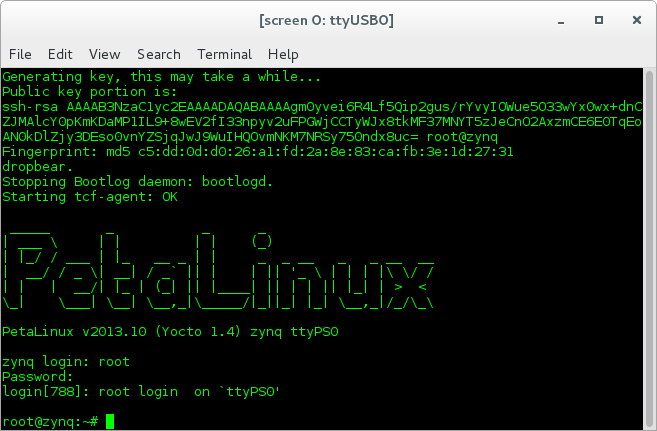
\includegraphics[scale=0.5]{Matchstiq_Z1_login}}
	\caption{Successful Boot to PetaLinux}
	\label{fig:boot1}
\end{figure}

\item Setup the OpenCPI environment on remote system

\begin{flushleft}
Each time the SDR is booted, the OpenCPI environment must be setup. By sourcing the \texttt{mynetsetup.sh} script, the remote system's environment is configured for OpenCPI and NFS directories are mounted for Network mode.\footnote{This script calls the \texttt{zynq\_net\_setup.sh} script, which should not be modifiable by the user.}. The user must provide the network address of the development system to the script as its only argument:
\begin{verbatim}
$ source /mnt/card/opencpi/mynetsetup.sh XX.XX.XX.XX
\end{verbatim} \medskip

where XX.XX.XX.XX is the IP address of the NFS host (i.e. that development host, \textit{e.g.} 192.168.1.10). A successful run is shown in Figure~\ref{fig:netsetup}.
\end{flushleft}

\begin{figure}[H]
	\centerline{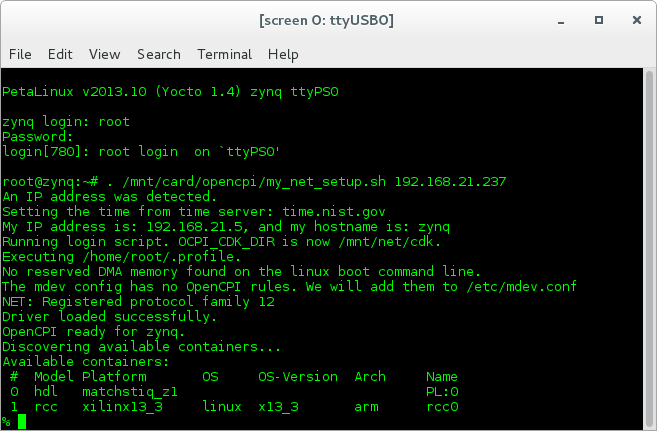
\includegraphics[scale=0.5]{Matchstiq_Z1_net_setup}}
	\caption{Successful Network Mode Setup}
	\label{fig:netsetup}
\end{figure} \medskip

\iffalse
This file is protected by Copyright. Please refer to the COPYRIGHT file
distributed with this source distribution.

This file is part of OpenCPI <http://www.opencpi.org>

OpenCPI is free software: you can redistribute it and/or modify it under the
terms of the GNU Lesser General Public License as published by the Free Software
Foundation, either version 3 of the License, or (at your option) any later
version.

OpenCPI is distributed in the hope that it will be useful, but WITHOUT ANY
WARRANTY; without even the implied warranty of MERCHANTABILITY or FITNESS FOR A
PARTICULAR PURPOSE. See the GNU Lesser General Public License for more details.

You should have received a copy of the GNU Lesser General Public License along
with this program. If not, see <http://www.gnu.org/licenses/>.
\fi

% This is for inserting into various "Getting Started" Guides
% It REQUIRES that "Setup_System_Time.tex" is also included.
\textit{Note}: If the output includes:
\begin{verbatim}
Attempting to set the time from time server
Alarm clock
\end{verbatim}
\path{ntp} was unable to set time using servers in \path{ntp.conf}. For more information see Section \ref{sec:Setup system time reference}


\end{enumerate}

\pagebreak
\subsection{Standalone Mode}
All artifacts (.so, .bit.gz) for any applications or tests that need to be located on the SD card must be on the ATLAS partition in the \texttt{opencpi/xilinx13\_3/artifacts} folder.  All of the helper utilities such as \texttt{ocpirun} and \texttt{ocpihdl} are already located on the SD card and do not need to be copied over to the SDR platform.

\begin{enumerate}
\item Ensure the USB to Ethernet adapter (as needed) is plugged into the micro-USB port of the front panel and connected to a network configured for DHCP. \item Ensure a micro-USB to USB cable is connected between the Matchstiq-Z1's serial port and development host.
\item Apply power to the Matchstiq-Z1
\item Use a serial terminal application to establish a serial connection, for example:

\begin{verbatim}
$ screen /dev/matchstiq_z1_0 115200
\end{verbatim} \medskip

\item After a successful boot to PetaLinux, login to the system, using  ``\textbf{root}`` for user name and password.

\begin{figure}[H]
	\centerline{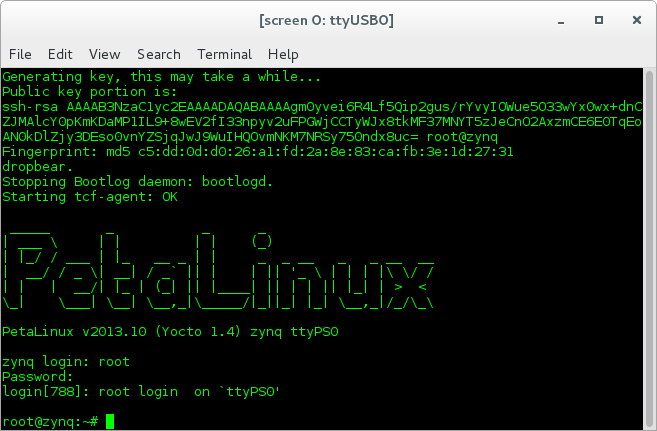
\includegraphics[scale=0.5]{Matchstiq_Z1_login}}
	\caption{Successful Boot}
	\label{fig:boot2}
\end{figure}

\item \textcolor{red}{WARNING:}
Applications (including XML-only ones) fail if there is not an IP address assigned to the platform, even when in ``standalone mode.'' When the Ethernet port is not connected to a network configured with DHCP, a temporary IP address must be set:
\begin{verbatim}
$ ifconfig eth0 192.168.244.244
\end{verbatim} \medskip

\item Setup the OpenCPI environment on remote system

Each time the SDR is booted, the OpenCPI environment must be setup. By sourcing the \texttt{mysetup.sh} script, the remote system's environment is configured for OpenCPI.\footnote{This script calls the \texttt{zynq\_setup.sh} script, which should not be modifiable by the user.}. There are no arguments required for this script.
\begin{verbatim}
$ source /mnt/card/opencpi/mysetup.sh
\end{verbatim} \medskip

\noindent A successful setup of the platform will look as follows:
\begin{figure}[H]
	\centerline{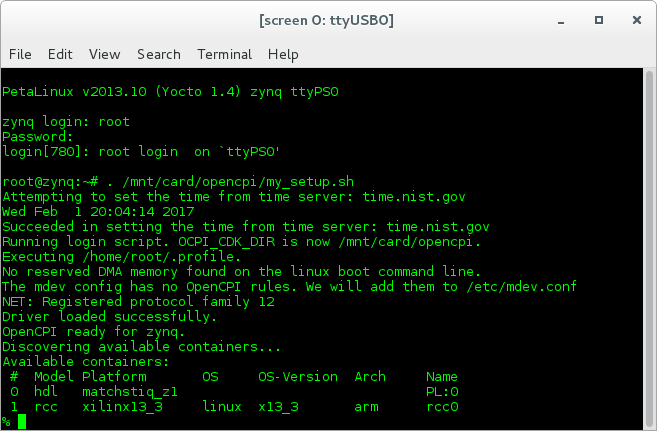
\includegraphics[scale=0.5]{Matchstiq_Z1_setup}}
	\caption{Successful Standalone Mode Setup}
	\label{fig:standalonesetup}
\end{figure} \medskip

\iffalse
This file is protected by Copyright. Please refer to the COPYRIGHT file
distributed with this source distribution.

This file is part of OpenCPI <http://www.opencpi.org>

OpenCPI is free software: you can redistribute it and/or modify it under the
terms of the GNU Lesser General Public License as published by the Free Software
Foundation, either version 3 of the License, or (at your option) any later
version.

OpenCPI is distributed in the hope that it will be useful, but WITHOUT ANY
WARRANTY; without even the implied warranty of MERCHANTABILITY or FITNESS FOR A
PARTICULAR PURPOSE. See the GNU Lesser General Public License for more details.

You should have received a copy of the GNU Lesser General Public License along
with this program. If not, see <http://www.gnu.org/licenses/>.
\fi

% This is for inserting into various "Getting Started" Guides
% It REQUIRES that "Setup_System_Time.tex" is also included.
\textit{Note}: If the output includes:
\begin{verbatim}
Attempting to set the time from time server
Alarm clock
\end{verbatim}
\path{ntp} was unable to set time using servers in \path{ntp.conf}. For more information see Section \ref{sec:Setup system time reference}


\end{enumerate}

\pagebreak
\section{Build an Application}
\begin{flushleft}
The setup of the platform can be verified by running an application that uses both RCC and HDL workers. A simple application that requires two RCC and one HDL worker is located in \texttt{assets/applications/bias.xml}, but only the RCC artifacts are provided with the installation of RPMs, and are availble on the SD card (Standard Mode) or mounted CDK directory (Network Mode). The remaining task is to build an assembly, or bitstream for loading the FPGA, which contains the HDL worker.
\end{flushleft}

\section{Run an Application}
\subsection{Network Mode}
The default setup script sets the \texttt{OCPI\_LIBRARY\_PATH} variable to include the RCC workers that are required to execute the application, but it must be updated to include to the assembly bitstream that was built.  After running the \texttt{mynetsetup.sh} script, navigate to  \texttt{/mnt/ocpi\_assets/applications}, then update the \texttt{OCPI\_LIBRARY\_PATH} variable:
\begin{verbatim}
$ cd /mnt/net/cdk/applications
$ export OCPI_LIBRARY_PATH=$OCPI_LIBRARY_PATH:/mnt/ocpi_assets/artifacts
\end{verbatim}
Run the application using the following command:
\begin{verbatim}
$ ocpirun -v -t 1 -d -m bias=hdl bias.xml
\end{verbatim}
The output should be similar to Figure~\ref{fig:netBias}:
\begin{verbatim}
% ocpirun -v -t 1 -d -m bias=hdl bias.xml
Available containers are:  0: PL:0 [model: hdl os:  platform:
matchstiq_z1], 1: rcc0 [model: rcc os: linux platform: xilinx13_3]
Actual deployment is:
  Instance  0 file_read (spec ocpi.core.file_read) on rcc container 1: rcc0, using file_read in
  /mnt/ocpi_core/artifacts/ocpi.core.file_read.rcc.0.xilinx13_3.so
  dated Tue Apr  9 11:34:43 2019
  Instance  1 bias (spec ocpi.core.bias) on hdl container 0: PL:0, using bias_vhdl/a/bias_vhdl in
  /mnt/ocpi_assets/applications/rx_app/../../artifacts/
  ocpi.assets.testbias_matchstiq_z1_base.hdl.0.matchstiq_z1.gz
  dated Mon Apr  8 14:31:34 2019
  Instance  2 file_write (spec ocpi.core.file_write) on rcc container 1: rcc0, using file_write in
  /mnt/ocpi_core/artifacts/ocpi.core.file_write.rcc.0.xilinx13_3.so
  dated Tue Apr  9 11:34:48 2019
Application XML parsed and deployments (containers and artifacts) chosen
Application established: containers, workers, connections all created
Communication with the application established
Dump of all initial property values:
Property  0: file_read.fileName = "test.input" (cached)
Property  1: file_read.messagesInFile = "false" (cached)
Property  2: file_read.opcode = "0" (cached)
Property  3: file_read.messageSize = "16"
Property  4: file_read.granularity = "4" (cached)
Property  5: file_read.repeat = "false"
Property  6: file_read.bytesRead = "0"
Property  7: file_read.messagesWritten = "0"
Property  8: file_read.suppressEOF = "false"
Property  9: file_read.badMessage = "false"
Property 10: file_read.ocpi_debug = "false" (parameter)
Property 11: file_read.ocpi_endian = "little" (parameter)
Property 16: bias.biasValue = "16909060" (cached)
Property 17: bias.ocpi_debug = "false" (parameter)
Property 18: bias.ocpi_endian = "little" (parameter)
Property 20: bias.test64 = "0"
Property 29: file_write.fileName = "test.output" (cached)
Property 30: file_write.messagesInFile = "false" (cached)
Property 31: file_write.bytesWritten = "0"
Property 32: file_write.messagesWritten = "0"
Property 33: file_write.stopOnEOF = "true" (cached)
Property 34: file_write.ocpi_debug = "false" (parameter)
Property 35: file_write.ocpi_endian = "little" (parameter)
Application started/running
Waiting up to 1 seconds for application to finish
Application is now considered finished after waiting 1 seconds
Dump of all final property values:
Property  3: file_read.messageSize = "16"
Property  6: file_read.bytesRead = "1776"
Property  7: file_read.messagesWritten = "111"
Property  9: file_read.badMessage = "false"
Property 31: file_write.bytesWritten = "1760"
Property 32: file_write.messagesWritten = "110"
\end{verbatim}

%\begin{figure}[H]
%	\centerline{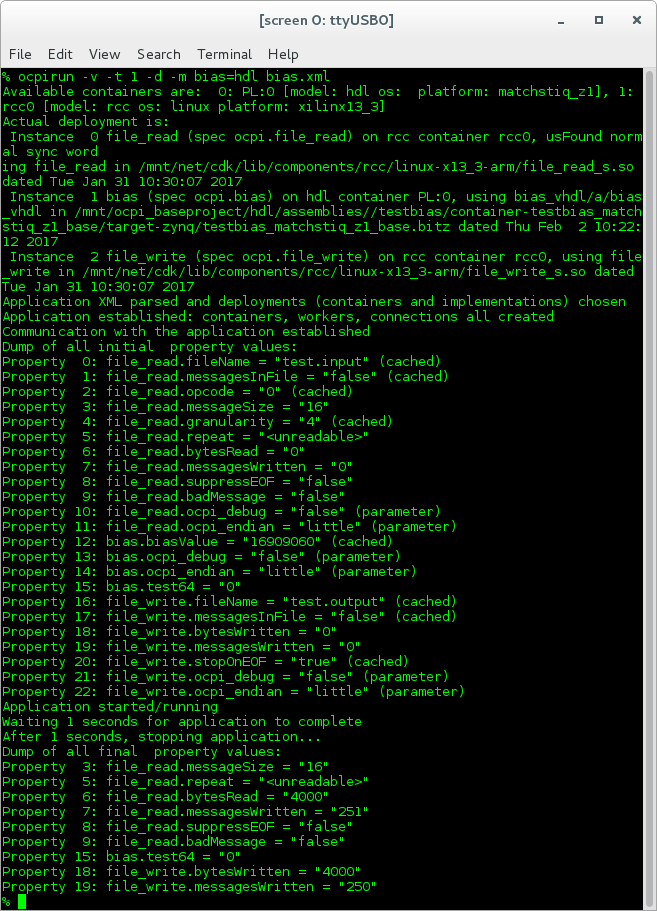
\includegraphics[scale=0.5]{Matchstiq_Z1_net_bias}}
%	\caption{Successful Network Mode Execution}
%	\label{fig:netBias}
%\end{figure}

\pagebreak
Run the following command to view the input. It should look like Figure~\ref{fig:inBias1}: \\
\begin{verbatim}
$ hexdump test.input | less
\end{verbatim}
\begin{figure}[H]
	\centerline{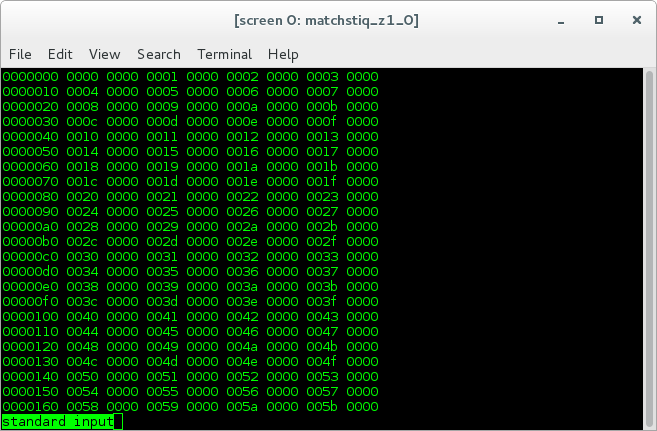
\includegraphics[scale=0.5]{Matchstiq_Z1_bias_input}}
	\caption{Expected Input}
	\label{fig:inBias1}
\end{figure}

Run the following command to view the output. It should look like Figure~\ref{fig:outBias1}: \\
\begin{verbatim}
$ hexdump test.output | less
\end{verbatim}
\begin{figure}[H]
	\centerline{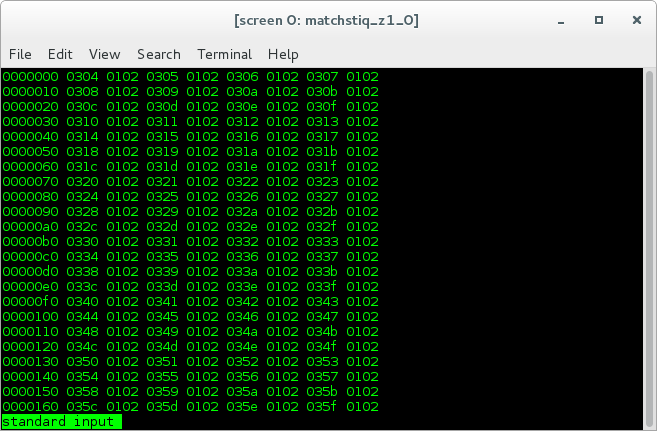
\includegraphics[scale=0.5]{Matchstiq_Z1_bias_output}}
	\caption{Expected Output}
	\label{fig:outBias1}
\end{figure}

\newpage
\subsection{Standalone Mode}
\begin{flushleft}
The default setup script sets the \texttt{OCPI\_LIBRARY\_PATH} variable to include the all of the artifacts that are required to execute the application. Specifically, all three of the artifacts that are located on the SD card are mounted at \texttt{/mnt/card/opencpi/xilinx13\_3/artifacts}.  After running \texttt{mysetup.sh}, navigate to \texttt{/mnt/card/opencpi/applications} and ensure the \texttt{OCPI\_LIBRARY\_PATH} variable is configure as shown below:
\begin{verbatim}
$ cd /mnt/card/opencpi/applications
$ export OCPI_LIBRARY_PATH=$OCPI_LIBRARY_PATH:/mnt/card/opencpi/xilinx13_3/artifacts
\end{verbatim}

Run the application using the following command:
\begin{verbatim}
$ ocpirun -v -t 1 -d -m bias=hdl bias.xml
\end{verbatim}
The output should be similar to Figure~\ref{fig:standBias}:
\end{flushleft}
\begin{figure}[H]
	\centerline{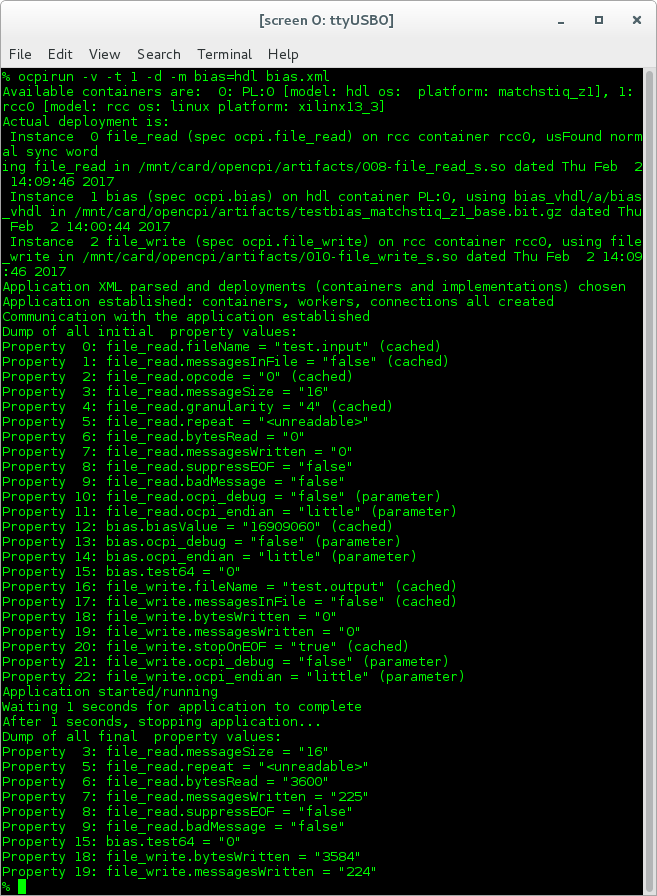
\includegraphics[scale=0.5]{Matchstiq_Z1_stand_bias}}
	\caption{Successful Standalone Mode Execution}
 \label{fig:standBias}
\end{figure}

\pagebreak
Run the following command to view the input. It should look like Figure~\ref{fig:inBias2}: \\
\begin{verbatim}
$ hexdump test.input | less
\end{verbatim}
\begin{figure}[H]
	\centerline{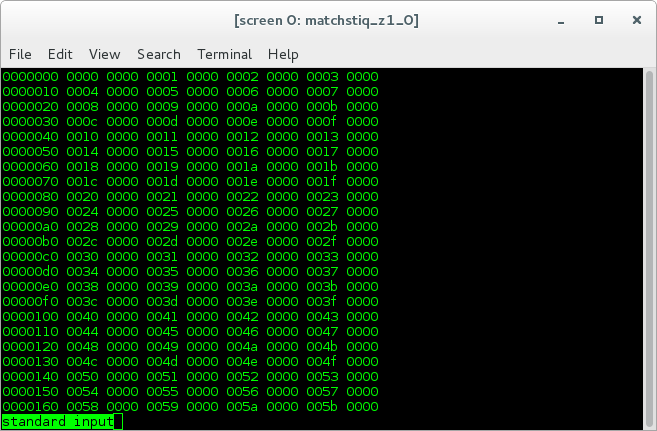
\includegraphics[scale=0.5]{Matchstiq_Z1_bias_input}}
	\caption{Expected Input}
	\label{fig:inBias2}
\end{figure}

Run the following command to view the output. It should look like Figure~\ref{fig:outBias2}: \\
\begin{verbatim}
$ hexdump test.output | less
\end{verbatim}
\begin{figure}[H]
	\centerline{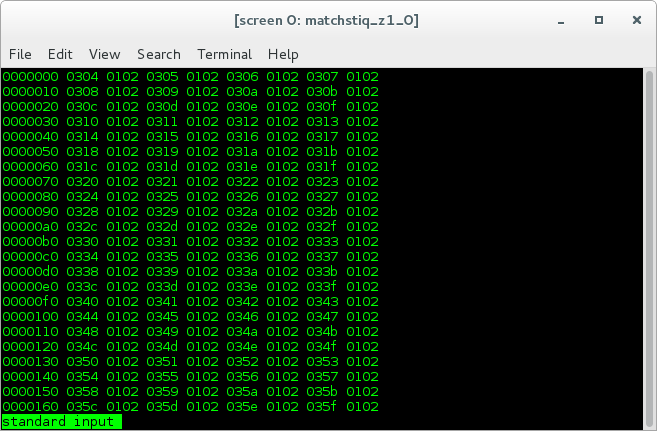
\includegraphics[scale=0.5]{Matchstiq_Z1_bias_output}}
	\caption{Expected Output}
	\label{fig:outBias2}
\end{figure}

\pagebreak
\begin{appendices}

\section{Intermittent Errors}
Some tests have had ``Segmentation Faults'' or ``Alignment Errors'' in certain scenarios on the Z1. This seems to happen when both USB ports are used to simultaneously transmit a large amount of data, \textit{e.g.} high log-level output to a USB serial console as well as NFS-mounted output files over a USB-to-Ethernet adapter. The default test setup avoids triggering this by limiting output that is fed to the user, but users should be aware of this issue if non-default test scenarios are attempted. If \texttt{ssh} is used to have all data routed through the USB-to-Ethernet adapter, this failure mode is avoided.
\section{Using ISE instead of Vivado with the Matchstiq-Z1}
It is recommended that you use the default toolset (Xilinx Vivado) to build Matchstiq-Z1 bitstreams with OpenCPI. However, if you wish to use ISE instead, reference the README file in \path{assets/hdl/platforms/matchstiq_z1/ise_constraints/}, and perform the following steps:
\begin{enumerate}
\item{Modify the target part in \path{assets/hdl/platforms/matchstiq_z1/matchstiq_z1.mk} to use the ISE alias:
\subitem \code{HdlPart\_matchstiq\_z1=xc7z020\_ise\_alias-1-clg484}}
\item{Export the ISE constraints files found in \path{<assets/>hdl/platforms/matchstiq_z1/ise_constraints/} by modifying \code{ExportFiles} variable in \path{assets/hdl/platforms/matchstiq_z1/Makefile}:
\subitem \code{ExportFiles=ise\_constraints/matchstiq\_z1.ucf ise\_constraints/matchstiq\_z1.ut matchstiq\_z1.mk}}
\end{enumerate}
% Bring in the kernel message snippet
\section{Driver Notes}
\iffalse
This file is protected by Copyright. Please refer to the COPYRIGHT file
distributed with this source distribution.

This file is part of OpenCPI <http://www.opencpi.org>

OpenCPI is free software: you can redistribute it and/or modify it under the
terms of the GNU Lesser General Public License as published by the Free Software
Foundation, either version 3 of the License, or (at your option) any later
version.

OpenCPI is distributed in the hope that it will be useful, but WITHOUT ANY
WARRANTY; without even the implied warranty of MERCHANTABILITY or FITNESS FOR A
PARTICULAR PURPOSE. See the GNU Lesser General Public License for more details.

You should have received a copy of the GNU Lesser General Public License along
with this program. If not, see <http://www.gnu.org/licenses/>.
\fi

% This is for inserting into various "Getting Started" Guides
% First, turn off indenting to avoid all the flushleft
\newlength{\savedparindentdrvr}%
\setlength{\savedparindentdrvr}{\parindent}%
\setlength{\parindent}{0pt} % Don't indent all paragraphs
\providecommand{\forceindent}{\leavevmode{\parindent=1em\indent}}%

When available, the driver will attempt to make use of the CMA region for direct memory access. In use cases where many memory allocations are made, the user may receive the following kernel message:

\lstset{language=bash, backgroundcolor=\color{lightgray}, columns=flexible, breaklines=true, prebreak=\textbackslash, basicstyle=\ttfamily, showstringspaces=false,upquote=true, aboveskip=\baselineskip, belowskip=\baselineskip}
\begin{lstlisting}
alloc_contig_range test_pages_isolated([memory start], [memory end]) failed
\end{lstlisting}

This is a kernel warning, but does not indicate that a memory allocation failure occurred, only that the CMA engine could not allocate memory in the first pass. Its default behavior is to make a second pass and if that succeeded the end user should not see any more error messages. An actual allocation failure will generate unambiguous error messages.

\setlength{\parindent}{\savedparindentdrvr}%

%
\end{appendices}
\end{document}
